\documentclass[11pt]{article}
\usepackage[T1]{fontenc}
\usepackage[utf8]{inputenc}
\usepackage{lmodern,microtype,xurl,seqsplit,upquote}
\usepackage[margin=1in]{geometry}
\usepackage{amsmath,amssymb,amsthm,booktabs,array,tabularx,longtable}
\usepackage{graphicx}
\usepackage[hidelinks]{hyperref}
\newcommand{\code}[1]{\texttt{#1}}
\newcommand{\longcode}[1]{\texttt{\seqsplit{#1}}}
\newcommand{\src}[2]{\href{https://github.com/jsmorph/leanexe/blob/4360920c3060d1c625b1860229b5116804d177c8/#1}{#2}}
\newcommand{\wgsrc}[2]{\href{https://github.com/jsmorph/leanexe/blob/9c7c7898ecae5f636cf1047142c8a68c1936e041/#1}{#2}}
\newcommand{\talossrc}[2]{\href{https://github.com/jsmorph/talos/blob/87e3aa5e8f6e6f3b3eb5e7e4c5aba43071002d47/#1}{#2}}
\newcolumntype{L}[1]{>{\raggedright\arraybackslash}p{#1}}
\newtheorem{theorem}{Theorem}
\newtheorem{definition}{Definition}
\emergencystretch=2em
\setcounter{tocdepth}{2}
\title{GPT-2 Inference from Lean to WebAssembly and WGSL:\\
Artifact Verification, Shader Proofs, and Execution Evidence}
\author{Jamie Stephens\thanks{Morphism (\url{https://morphism.com}).  Contact: \href{mailto:js@morphism.com}{js@morphism.com}.}}
\date{19 September 2026}
\hypersetup{pdftitle={GPT-2 Inference from Lean to WebAssembly and WGSL: Artifact Verification, Shader Proofs, and Execution Evidence},pdfauthor={Jamie Stephens},pdfsubject={Programming languages; formal verification; language-model inference}}

\begin{document}
\maketitle
\begin{abstract}
Executing a language model requires agreement between its algorithm, floating-point operations, tensor storage, compiled instructions, and retained state.  LeanExe addresses this problem by compiling a restricted subset of Lean and checking proofs about the emitted program.  We apply the method to GPT-2 with 124,439,808 parameters and a 128-token context.  For the CPU path, a Lean-checked theorem connects a 19,083-byte WebAssembly binary to the source cached-inference recurrence.  It proves termination and exact cache and logit bytes for every weight array of the required length and every valid token sequence of length at most 128.  The proof includes binary decoding, validation, scalar arithmetic, tensor loops, allocation, and buffer releases.  Talos, a WebAssembly interpreter and proof library written in Lean, supplies the execution semantics.  Our extensions define binary32 and binary64 arithmetic through integer operations and explicit rounding.  Wasmtime, a standalone WebAssembly runtime, executes the CPU module with arithmetic NaN canonicalization enabled.  For GPU execution, six kernels compiled to the WebGPU Shading Language (WGSL) replace matrix products while WebAssembly retains the controller and remaining model operations.  Checked source, parsing, statement-execution, and packed-layout equalities support a complete hybrid session theorem with explicit shader-execution and host-transfer premises.  We describe the theorem structure, proof reuse, deployment assumptions, and related verification results.  Recorded native tests compare every logit across 128 contexts.  A user-supplied browser run shows matching 32-token completions and a reported 15.72-fold increase in decode throughput with WGSL.  Its screenshots and measurement definitions document that observation.  The CPU binary theorem and the conditional hybrid theorem have distinct deployment boundaries, which the report states alongside the execution evidence.
\end{abstract}

\tableofcontents
\clearpage
\section{Goal, motivation, and results}
\label{sec:context}

\subsection{Source-defined language-model inference}

LeanExe's goal is to run an algorithm written in Lean with a checked proof that the emitted program implements that algorithm.  The source definition specifies the intended computation.  The compiled program supplies an execution path independent of Lean's runtime.  A per-artifact proof connects the target instructions, their memory operations, and their observable results to the chosen specification.  GPT-2 provides a case in which that connection must survive millions of floating-point operations, nested tensor loops, retained key/value state, and repeated allocation and release~\cite{subset,cached,entry}.

The initial practical objective was command-line inference with a pretrained language model and a complete source-agreement proof.  A user supplies a prompt, the host converts it into vocabulary indices, and the inference module returns the scores used to select subsequent tokens.  The implemented model has the block structure and parameter dimensions of GPT-2 124M, with an implemented context limit of 128 tokens.  Its weights arrive as runtime bytes.  The verification therefore applies to replacement weight values of the same shape without retraining or checking a new weight-specific theorem~\cite{manifest,guide,session}.

The algorithm fixes FP32 operation order and the numerical routines for normalization, exponentiation, and activation.  Equality with this source algorithm requires equality of represented words, including the specified exceptional results.  The verification target also includes successful execution: a proof of output equality conditional on a completed call would leave allocation failure and nontermination unresolved.  The session theorem combines these obligations and derives the memory conditions used by each token call from initialization~\cite{entry,session,budget}.

GPU execution introduces a second implementation of selected operations.  Matrix-product output coordinates can execute independently, while each coordinate retains its ordered accumulation.  The WGSL development moves those products to shaders and keeps the rest of the model in WebAssembly.  The resulting proof must connect three interfaces: the Lean kernel definition to emitted shader statements, the shader's input and output views to the packed model tensors, and the external call to the WebAssembly controller.  The conditional hybrid theorem composes these connections~\cite{wg-plan,wg-packedsource,wg-backend}.

\subsection{Two execution paths and their checked results}

The CPU artifact result starts with the complete frozen WebAssembly byte sequence.  Kernel-checked decoding and validation recover a module whose Talos translation equals the module used by the inference proof.  Talos is a WebAssembly interpreter and proof library written in Lean.  In its semantics, the recovered module terminates and returns the exact cache and logits of the Lean recurrence for every permitted session.  The public theorem is \longcode{Project.Gpt2CachedStep.Artifact.artifact\_gpt2\_128\_exact}~\cite{artifact}.

Wasmtime is the standalone WebAssembly runtime used for native CPU execution.  Its selected configuration canonicalizes arithmetic NaNs to agree with the formal word-level computation.  Application of the theorem to the running command trusts Wasmtime, the native host, and the association between file bytes and the embedded binary.  The recorded artifact check compares those bytes.  Section~\ref{sec:boundary} states the remaining runtime and automation assumptions~\cite{wasmtimeintro,wasmtime,artifactgate}.

The hybrid result starts with a modeled WebAssembly controller and six certified shader strings.  WGSL is the WebGPU Shading Language.  WebGPU supplies the API through which a host creates shader pipelines, submits work, and transfers buffers.  The checked shader results concern an explicit statement semantics for the supported grammar.  The complete hybrid theorem assumes that external calls complete according to that strict shader semantics, copy the specified bytes, and preserve the rest of the WebAssembly store.  Packed-layout theorems then identify those results with the CPU source operations.  The public hybrid session declarations include \code{gpt2\_128\_exact} and \code{gpt2\_128\_exact\_for} in namespace \code{Project.Gpt2Hybrid.Spec}~\cite{wg-execution,wg-backend,wg-composition}.

These two statements support different deployment claims.  The CPU proof includes the binary-to-model connection.  The hybrid proof includes a checked shader-to-source connection and an explicit external-execution premise.  The current hybrid binary enters the proof through declarations generated by an external parser.  Its native and browser hosts provide implementations of the required call sequence, and execution tests provide evidence about those implementations.  The theorem's explicit host premise and that empirical evidence remain separate~\cite{wg-build,wg-host,wg-review}.

\subsection{Execution evidence and report checkpoints}

The CPU test record compares 6,432,896 logits against PyTorch over one 128-token sequence and all its prefixes.  Every component meets the recorded tolerance, and the maximum observed absolute difference is approximately 0.001450.  The hybrid integration journal records the same number of exact logit comparisons against the parent WebAssembly path on a CPU WebGPU implementation.  The browser screenshots supplied for this report show both backends completing the same 32-token continuation.  The page reports a decode-throughput ratio of 15.72.  Sections~\ref{sec:tests} and~\ref{sec:browser} identify the populations, measurement rules, and provenance of these observations~\cite{tests,wg-journal}.

The CPU proof checkpoint is \longcode{4360920c3060d1c625b1860229b5116804d177c8}.  The WGSL and browser source checkpoint is \longcode{9c7c7898ecae5f636cf1047142c8a68c1936e041}.  Its two commits after the earlier WGSL report add the comparison page and focused worker tests.  They change host, interface, and documentation files.  The shader and inference proof sources retain the preceding reviewed development.  Both paths use Lean 4.34.0-rc2 at revision \longcode{6a10ac8c22beadecabdbb0919c2b50214762f91d} and Talos at revision \longcode{87e3aa5e8f6e6f3b3eb5e7e4c5aba43071002d47}~\cite{repo,wg-checkpoint,talos}.

This report combines and expands the CPU and WGSL technical reports~\cite{cpu-report,wg-report}.  It states the algorithm, proof subjects, execution assumptions, and measurements in one account.  The literature search compares complete artifact verification with source-level network reasoning, compiler transformations, and cryptographic certificates for inference evaluations.  The search found no earlier result with the same combination of a complete GPT-style inference module, proof-assistant-checked source agreement, and a checked connection from executable binary bytes.  The priority assessment is qualified by the search coverage described in Section~\ref{sec:related}.

\section{LeanExe: compilation and per-artifact verification}
\label{sec:leanexe}

\subsection{A checked Lean definition as an algorithm specification}

LeanExe imports an elaborated Lean declaration from a built module and compiles its reachable executable definitions.  Lean performs parsing, elaboration, type checking, and proof checking before LeanExe inspects the declaration.  The accepted runtime language is a restricted, pure, monomorphic, first-order subset with machine integers, bounded natural-number computations, packed byte arrays, supported array forms, structures, and internal recursive data.  Supported loops and helper calls express the model's numerical computation.  The language specification identifies accepted primitives and rejects residual expressions outside the subset~\cite{language,subset}.

The source definition supplies a precise specification because it fixes both control flow and arithmetic choices.  In GPT-2, this includes the order of each dot product, the offsets of runtime weight tensors, the byte representation of the cache, and the return value on an invalid input.  A mathematical description such as ``compute attention'' leaves these choices open.  The Lean definition resolves them, and the target proof uses the same definitions when stating expected results~\cite{cached,kernels,numerics}.

Lean's proof language can express richer predicates than the executable subset.  A theorem may quantify over arbitrary initial stores, describe ownership and disjointness, or compare an emitted computation with a mathematical recurrence.  Those proof expressions serve as specifications and evidence.  The compiler emits the runtime-relevant program after erasure of proof arguments and fields with no runtime content.  Its accepted-language checks constrain the computation that survives erasure~\cite{language}.

The theorem subject remains a particular program and specification.  The developer chooses the specification and reviews its meaning.  Lean's kernel checks whether the supplied proof has that type.  These two checks answer different questions: the source definition identifies the intended algorithm, and kernel checking establishes the formal implication.  The statement-review lemmas described later examine whether the public GPT-2 theorem entails concrete successful runs, the complete logit length, and the expected cache growth~\cite{reviewlemmas}.

\subsection{Compilation, representation, and ownership}

The compiler specializes supported source definitions, lowers them into a first-order intermediate representation, and emits structured WebAssembly instructions and their binary encoding.  It also emits WAT, WebAssembly's text format, for inspection.  A library-mode module exports its entry and memory-management functions.  Arrays and byte arrays become objects in linear memory with representations fixed by the ABI.  Scalar instructions and packed loads and stores implement the source primitives~\cite{language,compiler-implementation}.

Packed FP32 storage is central to the GPT-2 implementation.  A 124,439,808-word checkpoint occupies 497,759,232 bytes.  Keeping each value in four bytes permits the full model to fit within a 32-bit WebAssembly memory and provides byte-level views that host code can copy to GPU buffers.  Logical source values retain their \code{ByteArray} interface, while compiler-recognized word operations emit direct reads and construction loops.  The packed-memory proof relates the linear-memory bytes to the source array at every access~\cite{packed,manifest}.

Ownership information determines which allocations a generated operation may retain, return, or release.  The artifact proof checks the resulting memory behavior against representation and heap predicates.  A returned byte array carries both its content and the ownership facts needed by later calls.  The caller can release intermediate buffers only after establishing that the remaining live objects are disjoint from the released allocation.  GPT-2's block and session proofs use those facts to retain weights and current cache while freeing temporary vectors and obsolete cache objects~\cite{entry,budget,session}.

This treatment makes memory management part of functional correctness.  A correct numerical result stored at an invalid or reused pointer would fail the representation postcondition.  A release that overwrites a live tensor would fail the preservation predicate required by the next operation.  Allocation theorems account for either reuse of a suitable free block or growth within the represented memory capacity.  The top-level session derives the resource inequalities used by those alternatives~\cite{budget,input}.

\subsection{Proofs for a compilation}

LeanExe's artifact method proves behavior for an identified compiler output.  The compiler can produce code, annotations, and proposed structural equalities.  Each fact used by the final theorem must follow from checked definitions and proofs.  The current GPT-2 result therefore establishes correctness of its compilation without requiring a theorem quantifying over every possible compiler input~\cite{artifact,binary}.

The binary proof embeds the entire executable byte sequence in Lean.  A proved-sound decoder recovers a formal syntax tree, a proved-sound validator establishes the supported module's validity, and a translation maps that module to Talos.  A checked equality identifies the translated module with the declarations used by the execution proof.  The final theorem substitutes through that equality.  A parsing or translation discrepancy prevents the equality from closing and therefore prevents the artifact theorem from following~\cite{binary,artifact}.

The complete bytes and the file digest have different roles.  The theorem concerns the bytes as a Lean value.  SHA-256 identifies a file in records and helps compare published artifacts.  The proof's semantic conclusion follows from the full byte value, decoding, and execution theorem.  The command that applies the proof to an external file must still establish that the file contains those bytes.  The focused artifact checker performs that comparison~\cite{artifactgate}.

Per-compilation verification also permits implementation changes.  A changed compiler output creates a new proof obligation against the same source algorithm or a revised specification.  Shared arithmetic, memory, and control-flow lemmas can survive the change when their hypotheses remain applicable.  The WGSL development uses this property to replace matrix implementations, preserve proofs for unchanged functions, and reconstruct the controller proof around new call interfaces~\cite{wg-transport,wg-composition}.

\subsection{Annotations and reusable proof structure}

Generated target programs contain repeated instruction patterns for loads, stores, loops, allocation, and stack management.  Compiler annotations identify candidate regions and record their intended source role.  Checked region equalities establish that the instructions at those locations match a proved template.  The proof can then use a theorem about the template while preserving a connection to the emitted program.  The annotation supplies a proposed correspondence that must survive checking~\cite{annotations,proof-method}.

Shared loop rules express a source recurrence and the target state that realizes it.  An invariant may assert that the first $i$ output words are initialized, that an accumulator equals a source fold prefix, and that all protected input bytes retain their initial values.  The rule composes one verified body step through the loop and establishes the final result.  The GPT-2 range-fold rule also preserves an arbitrary operand-stack prefix, which is needed when a destination address remains on the stack during an inner reduction~\cite{loops}.

The repository's broader proof-generation tools use retrieved lemmas, tactics, and worked examples to propose proofs.  Compiler annotations and a structured knowledge library help select applicable material.  The proof-producing process may use coding agents, while the final check accepts Lean proof terms against the exact program and specification.  The GPT-2 proof described here uses the shared proof library and explicit component composition.  Its checked theorem depends on those accepted declarations~\cite{proof-method,ltg,entry}.

This architecture separates the cost of constructing a proof from the basis for accepting it.  An expensive search, a hand-written lemma, or an automatically generated application can produce the same checked proposition.  Reusable results reduce the amount of target-level reasoning needed for each new component.  In this development, scalar arithmetic, packed memory, allocator behavior, loop execution, and function-region transport provide the main reusable interfaces.  Architecture-specific theorems then compose them around fixed GPT-2 dimensions~\cite{f32,packed,budget,wg-transport}.

\subsection{Practical value and scope of the approach}

The result gives a precise answer to an implementation question: whether the emitted module executes the selected algorithm on every input in its specified domain.  It covers mistakes in arithmetic lowering, address calculations, control flow, cache assembly, and memory management when those mistakes would violate the source result or required successful execution.  A checkpoint change of the same byte length preserves the theorem's applicability because the weight values remain quantified inputs~\cite{session,artifact}.

The source remains available for algorithm review.  If a numerical method or cache convention in that source is unsuitable for an application, source agreement preserves that choice.  A separate numerical analysis can compare the source computation with real formulas, and a model evaluation can measure prediction quality.  The present GPT-2 work prioritizes exact implementation agreement.  PyTorch comparisons and text completions supply empirical evidence about the selected model and numerical methods~\cite{tests,testcode}.

The two backends show how the approach extends across execution interfaces.  The CPU path has a complete binary-to-source theorem within the formal WebAssembly semantics.  The shader path has per-compilation statement proofs and exact packed-layout equalities that compose under a host-execution premise.  The unresolved correspondence between physical shader execution and the strict arithmetic model determines the current limit of the GPU guarantee.  The proof records that premise where the external call enters the controller argument~\cite{wg-backend,wg-execution}.

\section{Lean algorithm and packed representation}
\label{sec:algorithm}

\subsection{Model dimensions and interface}

The implementation retains the original GPT-2 block organization: pre-normalized attention and feed-forward sublayers, residual additions, final normalization, and a vocabulary projection tied to the token embedding~\cite{gpt2}.  Table~\ref{tab:shape} gives the dimensions that determine loop bounds and buffer sizes.  The checkpoint contains 1,024 position embeddings, while the implemented cached entry accepts positions zero through 127~\cite{manifest,cached}.

\begin{table}[ht]
\centering
\begin{tabular}{lr}
\toprule
Quantity & Value\\
\midrule
Parameter words & 124,439,808\\
Transformer blocks & 12\\
Hidden width & 768\\
Attention heads & 12\\
Channels per head & 64\\
Feed-forward width & 3,072\\
Vocabulary size & 50,257\\
Supported context & 128 tokens\\
Weight payload & 497,759,232 bytes\\
One logit vector & 201,028 bytes\\
Cache increment per token & 73,728 bytes\\
\bottomrule
\end{tabular}
\caption{Dimensions used by the implementation and proof.}
\label{tab:shape}
\end{table}

A token is a vocabulary index represented by \code{UInt32}.  Context length counts these indices.  Weights, activations, cached keys and values, and logits use little-endian packed 32-bit words in Lean \code{ByteArray} values.  The source operations \code{word} and \code{generateUInt32LE} read and construct those words.  The compiler emits scalar FP32 instructions and packed memory operations for them~\cite{kernels,packed}.

The source entry has the type
\[
\code{ByteArray}\to\code{ByteArray}\to\code{UInt32}\to\code{Nat}\to\code{CachedResult}.
\]
Its arguments are weights, the prior cache, a token, and its position.  A \code{CachedResult} contains the extended cache and the next-token logit vector.  At position $p$, the entry checks weight length, token range, $p<128$, and cache length $73{,}728p$.  A failed check returns two empty byte arrays.  The separate rejected-entry theorem proves four zero result words and complete store preservation under the public entry's representation conditions~\cite{entry}.

The host API passes the weight pointer and byte length, cache pointer and byte length, token, and position, in that order.  The export returns cache pointer, cache byte length, logit pointer, and logit byte length.  Talos represents call arguments and results in operand-stack order, which reverses these lists.  Checked equalities identify \code{cachedStep}, \code{alloc}, \code{reset}, and \code{release} with function indices 38, 39, 40, and 42~\cite{initialize}.

\subsection{Cached attention and token recurrence}

The cache stores both 768-component key and value vectors for each layer and prior token.  Within a position, the twelve layers occur in increasing order, with keys preceding values in each layer.  If $s$ is a prior position, $\ell$ is a layer, and $o<1536$ selects a key or value component, its word index is
\[
((12s+\ell)1536)+o.
\]
For the current position, \code{cachedKv} reads the key or value from the newly computed QKV projection.  The source calculates attention scores by a 64-term ordered dot product, scales by $1/8$, normalizes over positions zero through the current position, and computes the weighted value sum~\cite{cached}.

Each block returns a new hidden vector and its current key/value vectors.  The enclosing twelve-layer loop concatenates those key/value vectors and appends them to the old cache.  Token and position embedding precede that loop.  Final layer normalization and the tied 50,257-row vocabulary projection follow it.  The cached Lean function specifies this entire token step.  The formal target takes its recurrence as the algorithm.  Comparison with the separate full-prefix implementation appears as a runtime test in Section~\ref{sec:tests}.

Let $W$ be a weight byte array and $t_0,\ldots,t_{n-1}$ the input tokens.  Define
\begin{equation}\label{eq:recurrence}
C_0=\epsilon,\qquad
(C_{p+1},L_p)=\code{cachedStep}(W,C_p,t_p,p),\quad 0\leq p<n,
\end{equation}
where $\epsilon$ is the empty byte array and $L_p$ is the logit byte array.  The Lean definition \code{Session.sourceTrace} returns the list of these cache/logit pairs.  Every equality to this trace is byte equality, so it includes signed zeros and the numerical routines' exceptional outputs.

\subsection{Arithmetic order and numerical routines}

Matrix projections accumulate each output component in source loop order, with a separate FP32 multiplication and addition at each step, followed by bias addition.  Layer normalization computes an ordered mean, an ordered sum of squared deviations, division by 768, addition of the FP32 word \code{0x3727C5AC} for epsilon, square root, and reciprocal.  It then applies the centered value, inverse standard deviation, scale, and bias in the written order~\cite{kernels}.  These choices determine the exact source result.

The source implements exponential evaluation by a degree-18 Horner polynomial with explicit coefficient words.  For finite nonpositive arguments, \code{expNeg} returns zero below $-64$, halves an argument below $-1$ at most six times, evaluates the polynomial, and squares the result once per halving.  GELU uses an exponential form of the tanh approximation and a magnitude cutoff at eight.  Beyond that cutoff, the finite positive tail returns the input and the finite negative tail returns zero~\cite{numerics}.  The bitwise comparisons and branch definitions in the cited source determine behavior on all other input words.  The execution proof includes those branches.

The polynomial, constants, cutoff tests, and rounding order form part of the algorithm specification.  The PyTorch reference uses its own tensor and transcendental implementations.  The report's numerical comparisons measure their agreement on the recorded checkpoint and token sequences.  Proving a real-valued approximation bound would require a separate statement relating these numerical routines to real formulas.

\subsection{Computation within a cached token step}

For each token, the source first adds its learned token embedding to its learned position embedding, component by component in FP32.  The resulting 768-word vector enters the twelve-block traversal.  Each block applies layer normalization to the current vector and then a linear projection with 2,304 output words.  These words contain query, key, and value vectors in that order, each of width 768.  Splitting each vector into twelve groups of 64 channels determines the attention heads~\cite{cached}.

For head $h$ and source position $s$, the score is an ordered 64-term dot product between the current query and the selected key, followed by multiplication by the binary32 word for $1/8$.  When $s$ precedes the current position, the key comes from the cache.  At the current position, it comes from the new projection.  The same selection rule applies to values.  Thus the current token participates in its attention computation before its key and value are appended to the retained cache~\cite{cached}.

Let $\oplus$, $\ominus$, $\otimes$, and $\oslash$ denote the source's specified word operations.  For a head with scores $a_0,\ldots,a_p$, the source computes a selected maximum $m$ through its comparison loop, then
\[
e_s=\operatorname{expNeg}(a_s\ominus m),\qquad
d=\operatorname{fold}_{s=0}^{p}(\oplus,e_s,0),\qquad
q_s=e_s\oslash d.
\]
The displayed fold denotes increasing-index accumulation from zero.  Each output channel then accumulates $q_s\otimes v_s$ in the same position order.  This notation abbreviates word functions and their branches, including exceptional encodings.  Their precise meaning comes from the Lean definitions~\cite{cached,numerics}.

The attention result undergoes a 768-to-768 projection and bias addition.  A residual addition combines that projection with the block input.  The block then applies its second layer normalization, a 768-to-3072 expansion, the selected GELU routine, and a 3072-to-768 projection.  A final residual addition gives the next hidden vector.  Separately, the block returns the 1,536 key/value words generated for this token~\cite{cached,kernels}.

The hidden traversal concatenates the twelve returned key/value arrays in layer order and appends the resulting per-token payload to the preceding cache.  Final layer normalization transforms the last hidden vector.  Vocabulary projection takes one ordered dot product against each of the 50,257 token-embedding rows.  This ties the output weights to the input token embedding.  The step returns the complete vocabulary-score array together with the new cache~\cite{cached,gpt2}.

Each stage has a corresponding execution-proof boundary.  Normalization and attention require scalar reductions and temporary buffers.  A linear projection requires matrix offsets, bias offsets, output construction, and ordered accumulation.  The block requires both output objects and cleanup.  The traversal requires a relation between the completed layer prefix and the assembled cache prefix.  These are the interfaces described in Section~\ref{sec:proof-structure}.  They align the target proof with the source's decomposition.

\section{CPU artifact theorem and floating-point semantics}

\subsection{Termination and observable results}

For a fixed Talos module $M$, environment $E$, function index $i$, initial store $S$, argument stack $a$, and postcondition $P$, write $\mathsf{TW}(E,M,i,S,a,P)$ for Talos's \code{TerminatesWith}.  Its definition is
\begin{equation}\label{eq:termination}
\exists N\;\forall f\geq N\;\exists v,S'.\quad
\code{run}(f,M,i,S,a,E)=\code{Success}(v,S')\ \land\ P(S',v).
\end{equation}
The natural number $f$ is interpreter fuel.  This predicate proves eventual successful execution and the postcondition for every sufficiently large fuel value~\cite{termination}.  The generated GPT-2 module has no imported functions, and the theorem quantifies over the host environment.

\begin{theorem}[Cached GPT-2 artifact execution]\label{thm:main}
Let $B$ be the frozen 19,083-byte artifact at the CPU proof checkpoint.  Decoding and validation succeed for $B$.  Its decoded module satisfies the formal binary grammar and validation rules of the supported profile.  Let $M$ be its Talos translation, $W$ a byte array of length $497{,}759{,}232$, and $T=[t_0,\ldots,t_{n-1}]$ a list of \code{UInt32} tokens with $n\leq128$ and $t_p<50{,}257$ for every $p<n$.  Starting from $M$'s initial store, reset and weight allocation terminate successfully.  After the specified byte copy of $W$ into the allocated payload, the token calls and releases described below terminate successfully.  At each position $p$, their observable cache and logit bytes equal $C_{p+1}$ and $L_p$ in Equation~\eqref{eq:recurrence}.
\end{theorem}

The checked declaration for Theorem~\ref{thm:main} is \longcode{Project.Gpt2CachedStep.Artifact.artifact\_gpt2\_128\_exact}~\cite{artifact}.  Its execution component transfers \longcode{Project.Gpt2CachedStep.Spec.gpt2\_128\_exact} to the decoded module~\cite{session}.  The three input conditions in the statement suffice, including for the empty token list.  For a nonempty list, \code{Session.RunsFor} calls \code{cachedStep}, observes the new cache, releases the previous cache when its pointer is nonzero, observes the logits, releases the logit buffer, and continues with the returned cache.  The step theorem preserves ownership of the weights and current cache through those releases.  The source trace specifies the outputs of this call sequence.

The weight-copy step is the pure store update \code{PackedInput.write}.  Its theorem establishes the required byte representation and heap ownership after allocation~\cite{input}.  This specifies the byte I/O boundary used by the execution theorem.  The native host performs the corresponding copy with \code{memcpy}.  The proof's trust boundary includes that implementation.

\subsection{Floating-point extensions to Talos}\label{sec:talosfp}

Our extensions give Talos executable binary32 and binary64 arithmetic definitions over integers and raw words.  The earlier evaluator stored floating-point values as \code{UInt32} and \code{UInt64} words, then called Lean's native \code{Float32} and \code{Float} operations to evaluate arithmetic~\cite{talosbefore}.  We added the \code{Wasm.IEEE32} and \code{Wasm.IEEE64} definitions and changed the interpreter's arithmetic dispatch to use them~\cite{talosfp,talosdispatch}.  These definitions expose the arithmetic computation to Lean proofs.

The models decode sign, exponent, and fraction fields.  Finite binary32 values have the form $z\,2^{-149}$ for an integer $z$, and finite binary64 values have the form $z\,2^{-1074}$.  Addition forms the exact integer sum at that scale.  Multiplication forms an exact dyadic product, and division forms an exact rational quotient.  Output rounding selects the nearest representable value and resolves ties toward an even significand.  The square-root implementation compares the exact radicand with a squared halfway point to choose the rounded result~\cite{talosfp}.  The integer definitions include subnormal values, gradual underflow, overflow, signed zeros, infinities, and canonical arithmetic NaNs.

The extension also gives integer definitions for comparisons, minimum and maximum, sign operations, rounding to an integer, and signed and unsigned integer conversions.  Trapping and saturating conversions have explicit range and exceptional-value branches.  Sign operations preserve the other word bits, including a NaN payload.  The big-step evaluator, small-step evaluator, and weakest-precondition rules use the corresponding arithmetic definitions and NaN classifiers~\cite{talosdispatch,talosfpproofs}.  At the pinned revision, cross-format promotion and demotion use Lean's conversion functions.  The generated GPT-2 module uses scalar binary32 arithmetic and raw-word reinterpretation.

We added operation theorems to Talos's CodeLib proof library for finite arithmetic, exceptional values, comparisons, rounding, and conversions.  For example, in namespace \code{CodeLib.IEEE32}, \code{mul\_finite\_rounder} identifies the product word with the dyadic rounder, and \code{sqrt\_signed\_zero} establishes the sign-preserving zero case.  Total execution theorems connect selected instruction sequences to these word functions, including multiplication, division, square root, conversion, and SIMD examples~\cite{talosfpproofs}.  The extension replaced the legacy \code{IEEE32Exec} compatibility axioms with proved equalities over the integer definitions~\cite{taloscompat}.

The extended library also contains real-error bounds under stated input conditions and proofs that compose rounding errors through Horner evaluation and dot products~\cite{talosnumeric}.  Those results support numerical analyses of floating-point algorithms.  The GPT-2 proof uses the exact operation definitions and execution rules, together with the source-correspondence equalities in the next subsection.  Talos supplies the arithmetic semantics.  The LeanExe proof workspace proves equality with Lean's logical \code{Float32} definitions for the five GPT-2 arithmetic operations on every input word.

\subsection{Arithmetic correspondence}

For each binary operation $\circ\in\{+,-,\times,/\}$, the arithmetic proof establishes
\[
\forall a,b:\code{UInt32},\qquad
\code{LeanExe.Float32.opBits}(a,b)
=\code{Wasm.IEEE32.op}(a,b).
\]
An analogous theorem covers square root.  Here \code{opBits} and \code{op} stand for the corresponding named operation.  The source intrinsics reduce to Lean's logical \code{Float32.Model}, and the proofs compare its encoding and rounding definitions with Talos's \code{IEEE32} operations~\cite{f32,leanfloat}.

The proofs split exceptional values from finite values, including zero and subnormal cases.  Shared lemmas relate encodings, significands, exponents, scaling, and rounding.  Finite multiplication, division, and square root require their respective rounding arguments.  NaN and infinity cases close against the explicit logical definitions.  The resulting equalities quantify over every input word and supply the scalar facts used by the tensor-loop proofs.  The formal source meaning comes from Lean's logical definitions.  Native Lean evaluation appears in separate execution tests.

\subsection{Allocation sufficiency through position 127}

The allocation proof bounds heap-top growth by charging each requested allocation, including alignment and allocator overhead.  A successful free-list reuse preserves the heap top, as does release.  Thus the argument applies to the existing allocator independently of which reusable block it selects~\cite{budget}.

Let $H_p$ be the heap top before token call $p$, and set
\[
B_0=536{,}870{,}912,\qquad D=16{,}777{,}216.
\]
These are 512 MiB and 16 MiB, respectively.  Initialization proves $H_0\leq B_0$.  The session invariant contains
\begin{equation}\label{eq:budget}
H_p\leq B_0+pD.
\end{equation}
For $p<128$ and a cache of length $73{,}728p$, \code{Entry.budget} proves every allocation-capacity premise and bounds the resulting heap top by $H_p+D$, provided $H_p+D<2^{32}$.  Equation~\eqref{eq:budget} supplies that premise because
\[
B_0+128D=2{,}684{,}354{,}560<2^{32}.
\]
The session induction therefore closes all 128 positions~\cite{budget,session}.

The memory invariant requires a 65,536-page capacity and bounds the page count by that capacity.  Each page contains 65,536 bytes, giving a 4 GiB memory bound.  The $2.5$ GiB expression above bounds the charged heap top.  The measured linear-memory size in Section~\ref{sec:tests} is a separate observation.  Host allocation success within the modeled capacity and sufficient native execution resources belong to the runtime assumptions.

\section{Artifact and runtime boundary}\label{sec:boundary}

\subsection{Binary decoding and execution transfer}

The artifact proof embeds all 19,083 bytes as the Lean value \code{artifactBytes}.  Checked parser certificates establish successful decoding of each function body, section, and the complete file.  The decoder soundness theorem connects that result to the declarative binary grammar.  Successful validation then yields \code{CoreValid}, which states section, memory-limit, global, export, and function-typing conditions for the supported binary profile~\cite{binary,artifact}.

The translation proof identifies each of the 43 decoded function bodies with the corresponding function in the execution model.  A whole-module equality also identifies types, exports, globals, memory, and the remaining module fields.  Equality substitution transfers the module-parameterized session specification \code{Spec.ExactSpecFor} to the decoded module~\cite{artifact,session}.  With $B=\code{artifactBytes}$, the final theorem has the form
\[
\begin{aligned}
\exists R,V.\quad
 &\code{decode}(B)=\code{ok}(R)\ \land\ \code{Grammar.Encodes}(B,R)\\
 &\land\ \code{validate}(R)=\code{ok}(V)\ \land\ \code{CoreValid}(R)\\
 &\land\ \code{ExactSpecFor}(V.\code{toTalos}).
\end{aligned}
\]
Here $R$ is the raw decoded module, $V$ is its validated representation, \code{Grammar.Encodes} is the declarative encoding relation, and \code{toTalos} is the formal translation.  \code{ExactSpecFor} states the initialization and session behavior in Theorem~\ref{thm:main}.  The compiler's output is the fixed subject of this proof.

The frozen artifact and the reviewed runtime binary have SHA-256
\begin{center}\small
\longcode{e93de126e00d7f5c5b9b30ca014a13b1385e9f91e3cb6b4e56a4aacf7a2b4ade}.
\end{center}
The package checker compares the external file with both the frozen package and the embedded byte array.  It then builds the artifact and behavior proofs, checks the registered artifact statements, and audits the registered declarations' axiom dependencies~\cite{artifactgate}.  A byte-for-byte comparison also confirmed the identity of the current command-line binary during the statement review~\cite{review}.  File reading and comparison connect the mathematical byte array to the file used for execution.

The source-driven check remains available: it recompiles \code{cachedStep}, renders the binary as WAT, generates a Talos module, and compares that module with the tracked execution model~\cite{gate}.  The recorded focused source check and exact-artifact check passed using the existing build cache~\cite{review}.  The runtime measurements in Section~\ref{sec:tests} retain the saved 18 September canonical-mode test record.

\subsection{Logical foundations}

The Lean kernel checks the proof terms.  The final artifact theorem's axiom report contains exactly \code{propext}, \code{Classical.choice}, and \code{Quot.sound}.  Propositional extensionality identifies logically equivalent propositions.  Choice selects an element from a type whose nonemptiness has been proved and supports classical reasoning.  Quotient soundness identifies quotient values represented by related elements.  These three principles supply the mathematical foundations used by the proof dependencies~\cite{leanaxioms,review}.

Native-evaluation axioms accept the result of a compiled computation and therefore add trust in the compiler and execution machinery used for that computation.  The generic package policy accepts these additional assumptions.  The statement review audited the final GPT-2 theorem against the three mathematical axioms~\cite{artifactgate,review}.

\subsection{Native execution}

WebAssembly permits multiple NaN results for some floating-point operations~\cite{wasmspec}.  Lean and Talos choose a canonical arithmetic NaN word, \code{0x7FC00000} for binary32.  The C host selects Cranelift and enables \longcode{wasmtime\_config\_cranelift\_nan\_canonicalization\_set}~\cite{wasmtime,driver}.  Wasmtime's implementation of that mode remains trusted.  The recorded FP32 tests check its exact NaN words, including signaling inputs and negative or noncanonical payloads~\cite{tests}.  The selected runtime mode is part of the deployment boundary for exact raw-word agreement.

The formal binary grammar, validation rules, translation, and Talos execution definitions specify the modeled WebAssembly behavior.  Applying their result to a native run trusts the correspondence of those definitions with WebAssembly, Wasmtime and its native-code backend, the C host, and the host's byte I/O.  Tokenization and token selection occur outside the proved recurrence.  The theorem accepts vocabulary indices and produces logit bytes, which lets either a user-selected sequence or a generated sequence supply the next valid token.


\section{Structure of the verification theorems and proofs}
\label{sec:proof-structure}

\subsection{Proof subjects and quantification}

The main result fixes a program while quantifying over its permitted data.  Its fixed objects include the architecture, the 128-token context limit, the packed layout, the numerical routines, and the emitted binary.  Its variable objects include every weight byte, every valid input token, and the token-list length within the limit.  This quantification explains why a new checkpoint of the required length preserves the theorem and why a changed architecture requires a new compiled artifact and corresponding proof~\cite{artifact,session}.

The source-step theorem and the initialized-session theorem expose different premises.  The former accepts an arbitrary represented store, a heap description, weight and cache pointers, a token, and a position.  It assumes that the input bytes occupy protected memory and supplies an allocation-resource condition when the source accepts the inputs.  The latter begins with the module's initial store, calls reset and allocation, performs the specified input-byte update, and derives the conditions needed by successive steps.  The session's public input restrictions reduce to weight length, token range, and token-count bound~\cite{entry,initialize,session}.

At the source level, the step function has a total return value for every Lean input.  Its acceptance checks select a complete inference result or two empty byte arrays.  At the target level, execution has explicit possibilities for traps and resource exhaustion.  The proof must establish a successful target result equal to the selected source value.  In the rejected branch, it proves the four zero return words and preservation of the store.  In the accepted branch, it establishes output allocation, contents, and ownership~\cite{entry}.

The CPU theorem quantifies over the formal host environment even though the checked module has no imported functions.  The hybrid module adds two external matrix imports.  Its theorem therefore uses an environment together with \code{PackedBackend.Host}, a proposition specifying those calls.  This is a semantic premise in the theorem's type.  The permitted logical axioms of the proof checker and the runtime premises of the proposition are separate parts of the assurance statement~\cite{artifact,wg-backend}.

\subsection{Successful execution and postcondition composition}

Equation~\eqref{eq:termination} gives the successful-execution meaning of \code{TerminatesWith}.  Its fuel threshold may depend on the invocation.  A wall-clock deadline or throughput rate would require a cost model relating interpreter steps to a runtime~\cite{termination}.

The proof library's monotonicity rule changes a proved postcondition into a weaker one.  Component proofs use it to expose exactly the facts required by a caller.  For example, a packed-output theorem may contain the final heap, ownership, frame preservation, page count, and output bytes.  A vocabulary caller can retain the ownership and bytes while hiding internal temporary allocations.  A session caller can then retain the next cache and observe the logits.  Each use is an implication between predicates that Lean checks~\cite{entry,session}.

The composition of two calls follows their execution order.  The first call's postcondition supplies the second call's store and premises.  This dependence is essential for retained state: the second token receives the cache returned by the first token in the memory that remains after the required releases.  A proof of two independent calls from unrelated stores would provide a different statement.  The recursive session predicate makes the shared state explicit~\cite{session}.

\subsection{The source trace and observable session}

The definition \code{Session.sourceTrace} recursively applies \code{cachedStep} to the weight array, next token, current position, and preceding result cache.  Its result is a list of \code{CachedResult} values.  The definition \code{Session.RunsFor} relates that list to calls of a selected WebAssembly module.  Its base case requires an empty result list when the token list is empty.  Its recursive case requires a successful token call, representation of the next cache, release of the previous cache, representation of the logits, release of the logit buffer, and the remaining session~\cite{session}.

This observation order establishes useful lifetime properties.  The new cache exists when the call returns.  The logits remain readable after releasing the previous cache.  Releasing the logits leaves a store from which the next token call can use the retained new cache.  The low-level ownership proofs justify these state transitions, and the public session predicate exposes the exact byte observations that result.  The final cache remains available after the last call because the recursive base case performs no further release~\cite{session}.

Talos records call arguments and results in operand-stack order.  The source entry's logical argument order is weights, cache, token, and position, with pointer/length pairs at the ABI.  The theorem lists stack values in the reversed order used by the interpreter.  Checked export identities establish which function index implements each public operation.  This resolves both a representational detail and a possible statement error: a theorem about the wrong index or argument order could prove a different invocation~\cite{initialize,reviewlemmas}.

The final source-agreement result is equality of all bytes at every observed step.  It includes every one of the 50,257 logits and the complete cache, which grows by 73,728 bytes per position.  A downstream sampling procedure may inspect those logits and choose the next valid token.  The theorem applies to any resulting finite token list within the supported limit.  Correctness of the procedure that chooses the list is an additional property of that procedure~\cite{session,reviewlemmas}.

\subsection{The invariant carried between token calls}

The \code{Session.Ready} structure packages the state needed to apply the token-step proof.  Table~\ref{tab:ready} groups its fields by purpose.  The invariant contains both representation and resource information, so the induction can establish a successful next call and retain a state suitable for its successor~\cite{session}.

\begin{table}[ht]
\centering\small
\begin{tabularx}{\linewidth}{L{0.23\linewidth}X}
\toprule
Invariant fields & Meaning at position $p$\\
\midrule
Heap and weight ownership & The store realizes the abstract heap and the weight allocation owns the supplied byte array of the required size.\\
Cache size and ownership & The cache has $73{,}728p$ bytes.  At position zero its pointer is zero.  At later positions it has a valid owned allocation.\\
Separation & At a positive position, weight and cache regions are disjoint.\\
Heap-top bound & The heap top is at most $536{,}870{,}912+p\,16{,}777{,}216$.\\
Pages and capacity & The page count is at most 65,536, and the modeled capacity is 65,536 pages.\\
\bottomrule
\end{tabularx}
\caption{The state invariant used by the complete session induction.}
\label{tab:ready}
\end{table}

Initialization proves \code{Ready} for an empty cache after reset, weight allocation, and input encoding.  The step lemma consumes \code{Ready} at position $p$, a valid token, and $p<128$.  It produces the exact source result and a continuation with \code{Ready} at $p+1$.  The list induction in \code{runs\_exact} applies that continuation to the remaining tokens.  The arithmetic fact $p+|T|\leq128$ supplies the position bound at each recursive call~\cite{session}.

The allocation estimate charges every requested allocation even when the allocator can reuse a free block.  This choice gives a monotone upper bound without requiring a particular free-list search outcome.  The proof still follows the implemented allocator: a successful reuse preserves the heap top, and growth consumes the charged budget.  The sufficient bound covers all positions through 127 and remains below the 32-bit address limit.  It gives a reusable interface between the tensor proof and allocator behavior~\cite{budget}.

\subsection{From arithmetic words to a complete transformer}

The lowest arithmetic equalities relate Lean's logical FP32 operations to Talos's integer-defined word operations.  Their variables are raw words.  Case analysis handles exceptional encodings, and finite cases establish the relevant rounding equality.  These results can be applied inside any supported tensor computation with the same operations.  Weight-specific inequalities are absent from their premises~\cite{f32,leanfloat}.

Packed-memory lemmas identify a source word with the four bytes read by emitted instructions.  Construction lemmas track the initialized prefix of a new byte array.  A loop invariant combines these representation facts with an arithmetic recurrence.  For a dot product, the target accumulator after $k$ iterations equals the source fold over indices below $k$.  The induction extends the prefix by one multiplication and one addition in the source order.  It also proves the addresses valid and retains the caller's protected memory~\cite{packed,loops}.

Tensor operations add a second level of composition.  Layer normalization combines mean, squared-deviation reduction, inverse standard deviation, scaling, and bias.  Cached attention combines key/value selection, scores, maximum and exponential normalization, and weighted values.  A transformer block combines these operations with four linear products, activation, residual additions, and the key/value result.  Temporary cleanup is checked before the block returns its outputs~\cite{entry}.

The hidden-state traversal iterates the block theorem across twelve layers.  Its invariant relates the hidden vector to the source traversal and the newly assembled per-token cache to the completed layers.  The proof separates layer execution, cache append, releases of temporary cache objects, releases of the prior hidden vector, and loop control.  This decomposition lets each stage use the ownership facts from the preceding stage and keeps the final traversal theorem expressed in terms of the source recurrence~\cite{entry}.

Vocabulary projection then computes all 50,257 scores from the final normalized hidden vector.  The accepted-entry theorem combines hidden traversal and projection, returns both allocated outputs, and proves preservation of protected inputs.  The complete entry theorem splits accepted and rejected inputs.  The session proof repeatedly invokes the accepted result after deriving its premises.  The artifact theorem finally changes the subject from the cached module declaration to the module recovered from the binary~\cite{entry,session,artifact}.

\begin{figure}[ht]
\centering\small
\begin{tabular}{c}
\fbox{\parbox{0.90\linewidth}{\centering Logical FP32 equalities and packed-memory representation}}\\[3pt]
$\Downarrow$\\[3pt]
\fbox{\parbox{0.90\linewidth}{\centering Ordered loop invariants, allocation, ownership, and frame preservation}}\\[3pt]
$\Downarrow$\\[3pt]
\fbox{\parbox{0.90\linewidth}{\centering Normalization, attention, linear products, activation, and residuals}}\\[3pt]
$\Downarrow$\\[3pt]
\fbox{\parbox{0.90\linewidth}{\centering Transformer block, twelve-layer traversal, cache assembly, vocabulary}}\\[3pt]
$\Downarrow$\\[3pt]
\fbox{\parbox{0.90\linewidth}{\centering Accepted/rejected entry and initialized 128-token session}}\\[3pt]
$\Downarrow$\\[3pt]
\fbox{\parbox{0.90\linewidth}{\centering Binary decoding and validation $+$ whole-module equality\\
imply the artifact execution theorem}}
\end{tabular}
\caption{The main proof dependencies.  Each level exposes result and memory facts for its caller.  The binary connection identifies the program to which the composed execution result applies.}
\label{fig:proof-structure}
\end{figure}

\subsection{Replacement proofs for hybrid execution}

The hybrid proof replaces a matrix call with a new implementation that satisfies the caller's required postcondition.  A shader certificate establishes invocation behavior for the emitted string.  A packed-layout proof connects the input views and serialized output to the parent's \code{linearRows} or \code{vocabularyHead} result.  The host hypothesis supplies completed external execution and the required byte transfer.  The wrapper theorem combines these facts with allocation and frame preservation~\cite{wg-packedshader,wg-backend}.

Unchanged helper functions form a closed call region.  Adding the two imports shifts their function indices.  \code{ImportShift} relates the old and new declarations and their renamed direct calls.  A semantic transport theorem preserves execution at each fuel value for functions inside the selected region.  The generator applies this result to existing helper theorems.  Controller segments that call the new matrix implementations are checked again with the replacement postconditions~\cite{wg-transport,wg-composition}.

The composition script prepares Lean source through namespace and index substitution.  Acceptance comes from rechecking the generated declarations against the parsed module and named theorem types.  The script records dependency identities and audits the public cached-step and session results.  A textual substitution that changes an instruction or theorem application inappropriately must still pass those checks.  The resulting hybrid statement carries the explicit host hypothesis through the complete session~\cite{wg-composition}.

\subsection{Review of the theorem's consequences}

The statement review checks consequences that make the public claim concrete.  \longcode{premises\_inhabited} constructs inputs satisfying the required lengths and ranges.  \code{every\_decoding\_has\_spec} transfers the result to every successful decode and validation of the frozen bytes.  \code{decoded\_export\_names} identifies the exported operations.  The trace-length and result-size lemmas establish one result per token, the cache-growth formula, and a complete vocabulary vector~\cite{reviewlemmas}.

\code{first\_token\_observation} derives explicit successful interpreter runs for reset, allocation, and the first inference call from the final artifact theorem.  Its conclusion gives output lengths and byte representations equal to the source result.  This examines the public theorem through an observable execution consequence.  The full list induction supplies the corresponding continuation through all permitted positions~\cite{reviewlemmas,session}.

The final axiom audit examines transitive proof dependencies.  The reviewed CPU artifact theorem and its seven consequence lemmas depend on \code{propext}, \code{Classical.choice}, and \code{Quot.sound}, or a subset.  A separate review of the proposition is still required: a checked implication can contain an unsatisfied runtime premise, and an axiom list reports neither its practical availability nor its intended meaning.  For the hybrid result, that proposition review identifies strict shader execution and host transfer as explicit remaining premises~\cite{review,wg-review}.

\section{Per-compilation shader certificates}

\subsection{Lean source subset}

The compiler accepts a monomorphic annotated Lean definition of type
\[
\code{ScalarArithmetic}\to(\mathbb N\to\code{UInt32})\to
(\mathbb N\to\code{UInt32})\to\mathbb N\to\mathbb N\to\code{UInt32}.
\]
The five arguments supply scalar operations, input buffers $A$ and $B$, and output coordinates.  A \code{UInt32} represents a floating-point word.  The \code{add} and \code{mul} fields of \code{ScalarArithmetic} specify its arithmetic~\cite{wg-compiler}.  For example, an ordered matrix cell is expressed by
\begin{verbatim}
@[wgsl] def matrix : Source.Kernel := fun ar a b row col =>
  Source.fold 4 0 fun k acc =>
    ar.add acc (ar.mul (a (row * 4 + k)) (b (k * 3 + col)))
\end{verbatim}
The definition's elaborated body determines the emitted computation.  Transparent helpers, word and index bindings, nested literal-count folds, finite word constants, buffer reads, addition, and multiplication belong to the supported subset.  Index expressions use naturals, coordinates, fold indices, addition, and multiplication.  The implementation bounds normalization and rejects unsupported residual expressions.  Runtime branches, dynamic iteration, barriers, atomics, and shared-memory communication lie outside this grammar~\cite{wg-compiler}.

Every fold count is at most 65,535.  Static access checks bound each index expression and its intermediate arithmetic, preventing u32 overflow and out-of-range reads.  Constants must encode finite binary32 values, including constants in unused bindings.  Input buffer words remain unrestricted.  The emitted wrapper declares two read-only storage buffers, a distinct output buffer, an $8\times8$ workgroup, an edge guard, and one output store per active invocation~\cite{wg-compiler,wg-execution}.

\subsection{Parsing, source equality, and execution}

The checker independently parses the emitted shader string into a statement program.  It checks the declarations, bindings, guard, loop initializer, comparison, increment, accumulator assignment, lexical scope, final store, and complete token consumption.  Parsed locals become indexed slots.  Bindings and loops remain statements in the syntax tree.  The parser accepts the compiler's restricted WGSL grammar~\cite{wg-compiler}.

For source function $f$, shader text $s$, parsed statement program $P$, and shape $S$, the compiler constructs three certificates:
\begin{gather}
\operatorname{parse}(s)=\operatorname{ok}(P),\label{eq:parse}\\
f=\operatorname{interpretSource}(P),\label{eq:source}\\
\operatorname{Implements}(s,S,f).\label{eq:implements}
\end{gather}
Equation~\eqref{eq:source} quantifies over both input buffers, both coordinates, and the scalar interpretation.  Its proof checks equality to the named Lean definition.  An incorrect arithmetic operator or a custom natural-number addition instance therefore has to satisfy the original source equality before the checker can accept the shader~\cite{wg-compiler}.

The \code{Implements} proposition quantifies over scalar interpretation $a$, memory $M$, output size $c$, and u32 coordinates $(r,q)$.  With adequate buffer lengths, it states
\[
\operatorname{runShader}(s,a,M,c,r,q)
=\operatorname{ok}(\operatorname{expected}(S,f,a,M,r,q)).
\]
For an active coordinate, \code{expected} is a write of $f(a,M.A,M.B,r,q)$ to $rS.\mathrm{cols}+q$.  For an inactive coordinate, it is no write.  The execution function can fail on a missing local, invalid load or store, or exhausted loop budget.  The theorem rules out each modeled failure~\cite{wg-execution}.

The shared proof establishes agreement between wrapping u32 index calculations and natural-number source indices within the validated bounds.  It then proves statement execution equal to source interpretation, including local bindings and scope restoration.  A loop tests its u32 counter, executes its body, assigns the accumulator, and increments the counter.  Its budget equals the literal count, and the proof establishes that the guard becomes false before an additional body execution is needed.  This is a successful-execution result with bounded termination~\cite{wg-execution}.

Checking finishes synchronously before files are emitted.  The parser reductions use kernel evaluation.  The compiler audits transitive dependencies of all three public certificates and permits only \code{propext}, \code{Classical.choice}, and \code{Quot.sound}.  It saves the shader, metadata, and Lean declarations that can be checked again independently of compilation.  The command \code{\#check\_wgsl} applies the same proof requirements to an existing shader file~\cite{wg-compiler}.  File reading and writing remain external operations around the theorem about the embedded string.

\subsection{Dispatch and arithmetic scope}

The body-compiler proof establishes one invocation's semantics.  Separate geometric lemmas prove coverage by the rounded-up dispatch and distinct output addresses for distinct active cells.  The operational model assumes read-only inputs and a separate output buffer.  A complete refinement to the WebGPU execution model, including an external scheduler, remains outside these certificates~\cite{wg-execution}.

The strict GPT-2 instantiation uses the pure Talos binary32 addition and multiplication functions, with source-ordered accumulation and separate rounding.  Its specification includes signed zeros, subnormals, and exceptional words.  WGSL permits implementation choices involving reassociation, fusion, subnormals, zero signs, and exceptional values~\cite{wg-wgsl}.  Applying the exact theorem to a runtime therefore requires more than acceptance of the shader by that runtime: execution must implement the stated operations and preserve the represented words through loads, copies, and stores.

The branch also contains an earlier fixed-template GEMM development.  That path proves termination and output correspondence under arbitrary interleavings in its own dispatch model, and supports separate or locally fused accumulation.  A fusion theorem characterizes each output by a sequence of explicit per-step choices.  Its numerical bounds and small-model mixed-precision experiments use additional domain premises~\cite{wg-legacy}.  The current body compiler has its own source and statement proofs.  Applying the older scheduler, fusion, and numerical results to the new grammar requires additional correspondence proofs.

\section{Connection to packed GPT-2 operations}

\subsection{Ordered products and byte layouts}

The current integration compiles six kernel definitions.  The four block products append bias words to their matrix input view and perform bias addition after the dot product.  Table~\ref{tab:kernels} gives the shapes, all with one output row~\cite{wg-packedsource}.

\begin{table}[ht]
\centering
\begin{tabular}{lrrc}
\toprule
Operation & Inner dimension & Output columns & Final bias\\
\midrule
QKV projection & 768 & 2304 & Yes\\
Attention projection & 768 & 768 & Yes\\
Feed-forward expansion & 768 & 3072 & Yes\\
Feed-forward projection & 3072 & 768 & Yes\\
Vocabulary, first slice & 768 & 25129 & No\\
Vocabulary, second slice & 768 & 25128 & No\\
\bottomrule
\end{tabular}
\caption{Shader roles in each cached token step.  The four block roles repeat across twelve blocks.}
\label{tab:kernels}
\end{table}

Let $\operatorname{word}(W,i)$ read word $i$ from packed byte array $W$.  For matrix offset $o$, bias offset $b$, inner dimension $K$, and column count $N$, the shader's second input view is
\[
B(i)=\begin{cases}
\operatorname{word}(W,o+i),&i<KN,\\
\operatorname{word}(W,b+i-KN),&i\geq KN.
\end{cases}
\]
The source proof identifies the reads at $kN+q$ with the parent's matrix reads, and the read at $KN+q$ with its bias.  Induction over the fold proves equality to the parent's ordered dot-product prefix.  A separate arithmetic equality connects the Lean source's logical FP32 operations to the pure Talos operations for all input words~\cite{wg-packedsource}.

The tied token embedding is vocabulary-major in the parent weights.  A vocabulary shader uses the transposed view
\[
B_s(kN+q)=\operatorname{word}(W,(s+q)768+k),
\]
with $(s,N)=(0,25129)$ or $(25129,25128)$.  The split assigns each vocabulary column to one complete 768-term dot product.  The composition theorem selects its shader, local column, and shifted output address, preserving the operation order within every dot product~\cite{wg-packedsource}.

The resulting theorems \code{biasedBytes\_exact} and \code{vocabularyBytes\_exact} identify serialized shader results with the parent's \code{linearRows} and \code{vocabularyHead} byte arrays.  The serializer's total definition maps an unsuccessful shader result to a default word.  The preceding per-column theorem proves success at every serialized column, so the byte equality eliminates that default case~\cite{wg-packedshader}.  These are equalities of word and byte computations without weight-magnitude premises.

\subsection{Host imports and controller reuse}

The hybrid module adds imports \code{wgsl.linear} and \code{wgsl.vocabulary}.  Its Wasm wrappers allocate packed output storage and call the imports.  Function indices shift by two.  The proof generator checks the wrappers and unchanged function declarations against the independently parsed hybrid module~\cite{wg-build,wg-backend}.

The reusable \code{ImportShift} relation identifies a closed set of unchanged functions, their renamed direct calls, and the memory declaration.  Its semantic transport theorem preserves interpreter execution at every fuel value and therefore transports the parent's total-correctness statements.  Functions in the selected set cannot call the changed matrix implementations.  Controller segments outside that set are checked again, with the replacement matrix theorems at their call sites~\cite{wg-transport,wg-composition}.

The interface \code{PackedBackend.Kernels} contains the six shader texts and their \code{Implements} proofs.  \code{PackedBackend.Code} identifies the wrappers, allocator, memory mode, and imports in the module.  \code{PackedBackend.Host} specifies what the external calls do.  For represented and protected input buffers with adequate sizes and allocation resources, it requires the host to return the modeled shader-output bytes in the allocated output and preserve the remaining store~\cite{wg-backend}.

The host premise concerns execution of the certified shader semantics.  Equality of those shader bytes to the parent matrix result follows from the packed-layout and arithmetic theorems.  Combining the two establishes exact returned lengths and bytes, ownership of the output, preservation of protected memory, heap validity, and memory-capacity preservation.  Those postconditions supply the parent's controller proofs with the facts needed for subsequent calls and releases~\cite{wg-packedshader,wg-backend}.


\section{Conditional session theorem and deployment boundary}
\label{sec:hybrid}

Let $W$ be any 497,759,232-byte array and let $t_0,\ldots,t_{n-1}$ satisfy $t_i<50257$ and $n\leq128$.  Define the source trace by
\[
C_0=\epsilon,\qquad (C_{i+1},L_i)=\code{cachedStep}(W,C_i,t_i,i).
\]
Here $\epsilon$ is the empty cache, and $L_i$ is the complete logit byte array.  Under \code{PackedBackend.Host}, the generated \code{gpt2\_128\_exact} theorem composes reset, weight allocation, the mathematical write of $W$, successive inference calls, logit availability, and releases with this source trace.  Its session predicate observes cache and logit bytes in memory.  Its call predicate, \code{TerminatesWith}, requires success for every sufficiently large interpreter fuel~\cite{wg-composition,wg-session}.

The session derives its heap and buffer preconditions from initialization and preserves them across token calls.  The cached-step proof also covers rejected input lengths, token IDs, and positions.  The algorithm uses arbitrary weight words, including exceptional encodings.  Consequently, the host premise must hold for the corresponding strict word semantics if the theorem is applied on that full domain.  The source theorem supplies no assertion that a particular GPU satisfies this premise on all weight arrays.

Wasmtime is the standalone WebAssembly runtime used by the native host.  The host enables its Cranelift arithmetic NaN canonicalization mode, as in the parent implementation.  Native WebGPU dispatch and readback finish before an import returns to Wasm.  GPU weight views use the matrix offsets passed by Wasm, and the host invalidates cached views after overlapping external writes or reset.  A model session uses fifty matrix views~\cite{wg-host}.

The browser implementation runs Wasm in a worker.  Each import copies input words to shared staging, sends a dispatch request, and waits for completion notification.  The WebGPU host writes result bytes to staging before waking the worker.  Each browser run creates its own host and copies the same weight bytes into Wasm and the host's source buffer.  Section~\ref{sec:browser} describes the supplied browser execution images and the worker test evidence~\cite{wg-host,wg-journal}.

Tokenization, sampling, and the FP32-to-FP64 adapter that presents logit words to the Wasm sampler lie outside the inference theorem~\cite{wg-build}.

The hybrid theorem's axiom audit permits the same three standard logical axioms as the parent.  Its explicit \code{Host} hypothesis is additional to that logical axiom list.  An axiom audit alone cannot discharge the hypothesis~\cite{wg-composition}.


\section{PyTorch comparisons and command-line inference}\label{sec:tests}
\subsection{CPU WebAssembly comparisons}

The runtime tests use the pinned pretrained checkpoint with CPU PyTorch 2.9.1 and Transformers 4.57.6.  The manifest checks model files by hash and records checkpoint revision \longcode{607a30d783dfa663caf39e06633721c8d4cfcd7e}~\cite{manifest}.  The CPU reference uses FP32, eager attention, and one PyTorch thread.  The WASM driver keeps weights and cached key/value data in a resident Wasmtime instance~\cite{driver}.

The 128-position test starts with the story prompt ``Once upon a time, in a small village'' and appends repetitions of a fixed sentence before taking the first 128 token IDs.  For each prefix length from one to 128, it compares all 50,257 cached WASM logits with the corresponding CPU PyTorch logits~\cite{testcode}.  This gives $128\times50{,}257=6{,}432{,}896$ comparisons.  Every component satisfies the test tolerance
\[
|\ell_{\rm wasm}-\ell_{\rm torch}|
\leq 0.002+10^{-4}|\ell_{\rm torch}|.
\]
The maximum observed absolute difference is approximately $0.001450$~\cite{tests}.  The quantified exact-equality theorem concerns the Lean source, while this tolerance test concerns the checkpoint and sequence just described.

The canonical-mode run took 100.2 seconds and reached approximately 1.03 GiB of WASM linear memory.  Its allocation counters recorded 33,025 allocations and 33,023 frees, leaving the weights and current cache.  The allocator reuses whole freed blocks.  The final cache contains $128\times73{,}728=9{,}437{,}184$ payload bytes.  The test also checks the four rejected-input conditions, cache reset and replay, and byte-exact agreement between cached and full-prefix WASM logits for the nine-token story prompt~\cite{tests,testcode}.  These timings describe the recorded local runs and support execution feasibility.  They provide no cross-system speed comparison.

Three recorded completions generated 64, 32, and 16 tokens in 55.6, 27.8, and 15.4 seconds.  The 16-token greedy completion matched PyTorch's token sequence.  The 64-token sampled completion began:
\begin{quote}
Once upon a time, in a small village called Hukur. The village is a great expanse of white sand and the winds blow fast
\end{quote}
The saved test record includes the complete strings and generation settings~\cite{tests}.  They demonstrate the command-line path from tokenizer output through the resident WASM module and back to text.

\subsection{CPU execution and proof-check commands}

From a prepared repository checkout, the WASM and PyTorch commands are:
\begin{quote}\small\ttfamily
\verb|tools/gpt2 --text 'Once upon a time' --generate 32 --seed 42|

\verb|tools/gpt2-pytorch --text 'Once upon a time' --generate 32 --seed 42|
\end{quote}
Both use a shared uv project with pinned Python dependencies.  The default generation settings are top-$k$ 40, temperature 0.8, and seed 42.  The WASM client uses the Lean SplitMix64 generator for random draws and Python for sampling probabilities.  PyTorch uses its own seeded generator, so equal seeds produce different draw sequences.  Adding \verb|--top-k 1| to each command selects greedy decoding.  Small logit differences can still change an argmax~\cite{driver}.

The setup command
\begin{quote}\small\ttfamily
\verb|uv run --project training/gpt2 training/gpt2/reference.py fetch|
\end{quote}
downloads and checks the checkpoint.  The reproduction guide lists the compiler and Wasmtime prerequisites~\cite{guide}.  After a WASM command has produced \longcode{build/gpt2-124m/inference/cachedStep.wasm}, the focused artifact check is
\begin{quote}\small\ttfamily
\verb|tools/artifact-proof.js check \|\\
\verb|  build/gpt2-124m/inference/cachedStep.wasm \|\\
\verb|  Project.Gpt2CachedStep.ArtifactTranslation|
\end{quote}
This check enforces binary identity as well as the registered proof checks.  The separate statement review and final-theorem axiom audit run with
\begin{quote}\small\ttfamily
\verb|tools/leanrun --timeout 3m lake -d proofs/talos/lean env lean \|\\
\verb|  proofs/talos/reviews/gpt2-2026-09-19.lean|
\end{quote}
The source-regeneration and numerical-comparison commands are
\begin{quote}\small\ttfamily
\verb|tools/talos-proof.js check gpt2_cached_step|

\verb|node test/packed.js --gpt2-cached --gpt2-completions|
\end{quote}

\subsection{Native hybrid comparisons}

The WGSL integration journal records execution of the pretrained checkpoint on SwiftShader's CPU WebGPU device.  Across a forced 128-token sequence, all 6,432,896 candidate logit words matched the parent Wasm outputs.  Complete cache arrays matched at positions 0, 1, 126, and 127.  Invalid-input tests preserved allocator statistics and memory size, and cache restart tests reproduced the outputs.  The comparison code tests equality of the words~\cite{wg-journal,wg-tests}.

The same record reports agreement with PyTorch of all 128 argmax choices and a maximum absolute logit difference of approximately 0.001541.  Every logit satisfied the tolerance $0.002+0.0001|\text{reference}|$.  The combined parent, hybrid, and reference comparison took approximately 114 seconds.  The CPU-only and hybrid records describe different recorded test runs, so their elapsed times and maximum differences retain their respective provenance~\cite{wg-journal,wg-tests,tests}.

The journal also records greedy text completions and a sampled parent/hybrid pair using the same Wasm tokenizer and sampler, temperature 0.8, and seed 42.  The sampled text and logged logit bytes matched.  The rebuilt source bundle reproduced those traces and passed focused tokenizer, sampler, and invalid-request tests.  These execution checks cover auxiliary components around the formal inference interface~\cite{wg-journal}.

The branch records eleven body-compiler examples with three certificates each and 63 exact CPU WebGPU output checks.  Twenty-four rejection cases cover unsupported source constructs, invalid dimensions and accesses, non-finite constants, changed operations, altered loops, and malformed stores.  These checks examine the dependence of the certificate on source operations and rejection of unsupported or inconsistent programs~\cite{wg-bodytests}.

\section{Browser comparison and user-supplied execution images}
\label{sec:browser}

\subsection{Shared model and generation path}

The current WGSL branch serves a comparison page with two backends: CPU WebAssembly and WebAssembly with WGSL matrix products.  Both use the same checkpoint, Wasm tokenizer, Wasm sampler, FP32-to-FP64 sampling adapter, and generation loop.  The CPU choice loads \code{model-cpu.wasm}, the unchanged parent module copied into the bundle.  The WGSL choice loads the hybrid \code{model.wasm} and six shader files.  The comparison action runs CPU WebAssembly first and WGSL second with the same prompt and settings~\cite{browser-source,wg-packedguide}.

Each run creates a worker.  The hybrid path also creates a WebGPU device and shared transfer staging.  The worker performs model calls and keeps the weights and cache in the module's linear memory.  When a matrix import runs, it copies the input vector to staging and posts the requested matrix role and weight offsets.  The host dispatches a shader, reads its output, copies the bytes to staging, and signals the worker.  The worker resumes after the completion signal and copies those bytes into the allocated Wasm result.  This implements a synchronous import over the browser's asynchronous GPU API~\cite{browser-source}.

The GPU host prepares raw-word weight views on demand.  A linear view appends the bias vector to its matrix words.  A vocabulary view transposes the tied embedding slice into the shader's expected indexing.  Those operations rearrange bytes and words.  Model arithmetic executes in the Wasm module and shaders.  The host retains the views for later token calls and destroys the device when the run ends.  The model uses fifty views: four for each of twelve layers and two for the vocabulary slices~\cite{browser-source,wg-packedsource}.

The page compares generated token IDs and the stopping reason.  It retains both displayed completions and reports whether they agree.  At temperature zero the shared sampler selects greedily.  The visible seed remains part of the settings, while the greedy path determines the displayed run's selection rule.  Matching token IDs establishes that the two paths selected the same continuation on that run.  The visible comparison records token agreement.  Exact logit equality remains a separate test property~\cite{browser-source,wg-packedguide}.

\subsection{Completion shown in the first image}

Figure~\ref{fig:browser-completion} reproduces \code{gpt-1.png}, supplied by Jamie Stephens on 19 September 2026 after a run of the WGSL branch web demonstration.  The prompt is
\begin{quote}
[Bad fiction contest] It was a dark and stormy night as
\end{quote}
The requested completion length is 32 tokens, the temperature is zero, and the seed is 42.  The selected WebGPU option is ``Available GPU.''  The displayed adapter identifies vendor \code{apple} and architecture \code{metal-3}.  These labels identify the API-reported adapter information visible in the screenshot.  The screenshot provenance record accompanies the image file~\cite{screenshots}.

Both result panes show the same continuation:
\begin{quote}
we were walking down the street. I was standing in the middle of the street, and I saw a man with a gun. I thought, 'What the
\end{quote}
The page reports that both runs finished after 32 generated tokens because the requested count was reached.  The continuation therefore ends at the generation limit shown by the interface.  It demonstrates execution through model calls, token selection, and text decoding for this prompt.  The formal inference result addresses the model's cache and logits at the encoded-token interface described earlier.

\begin{figure}[p]
\centering
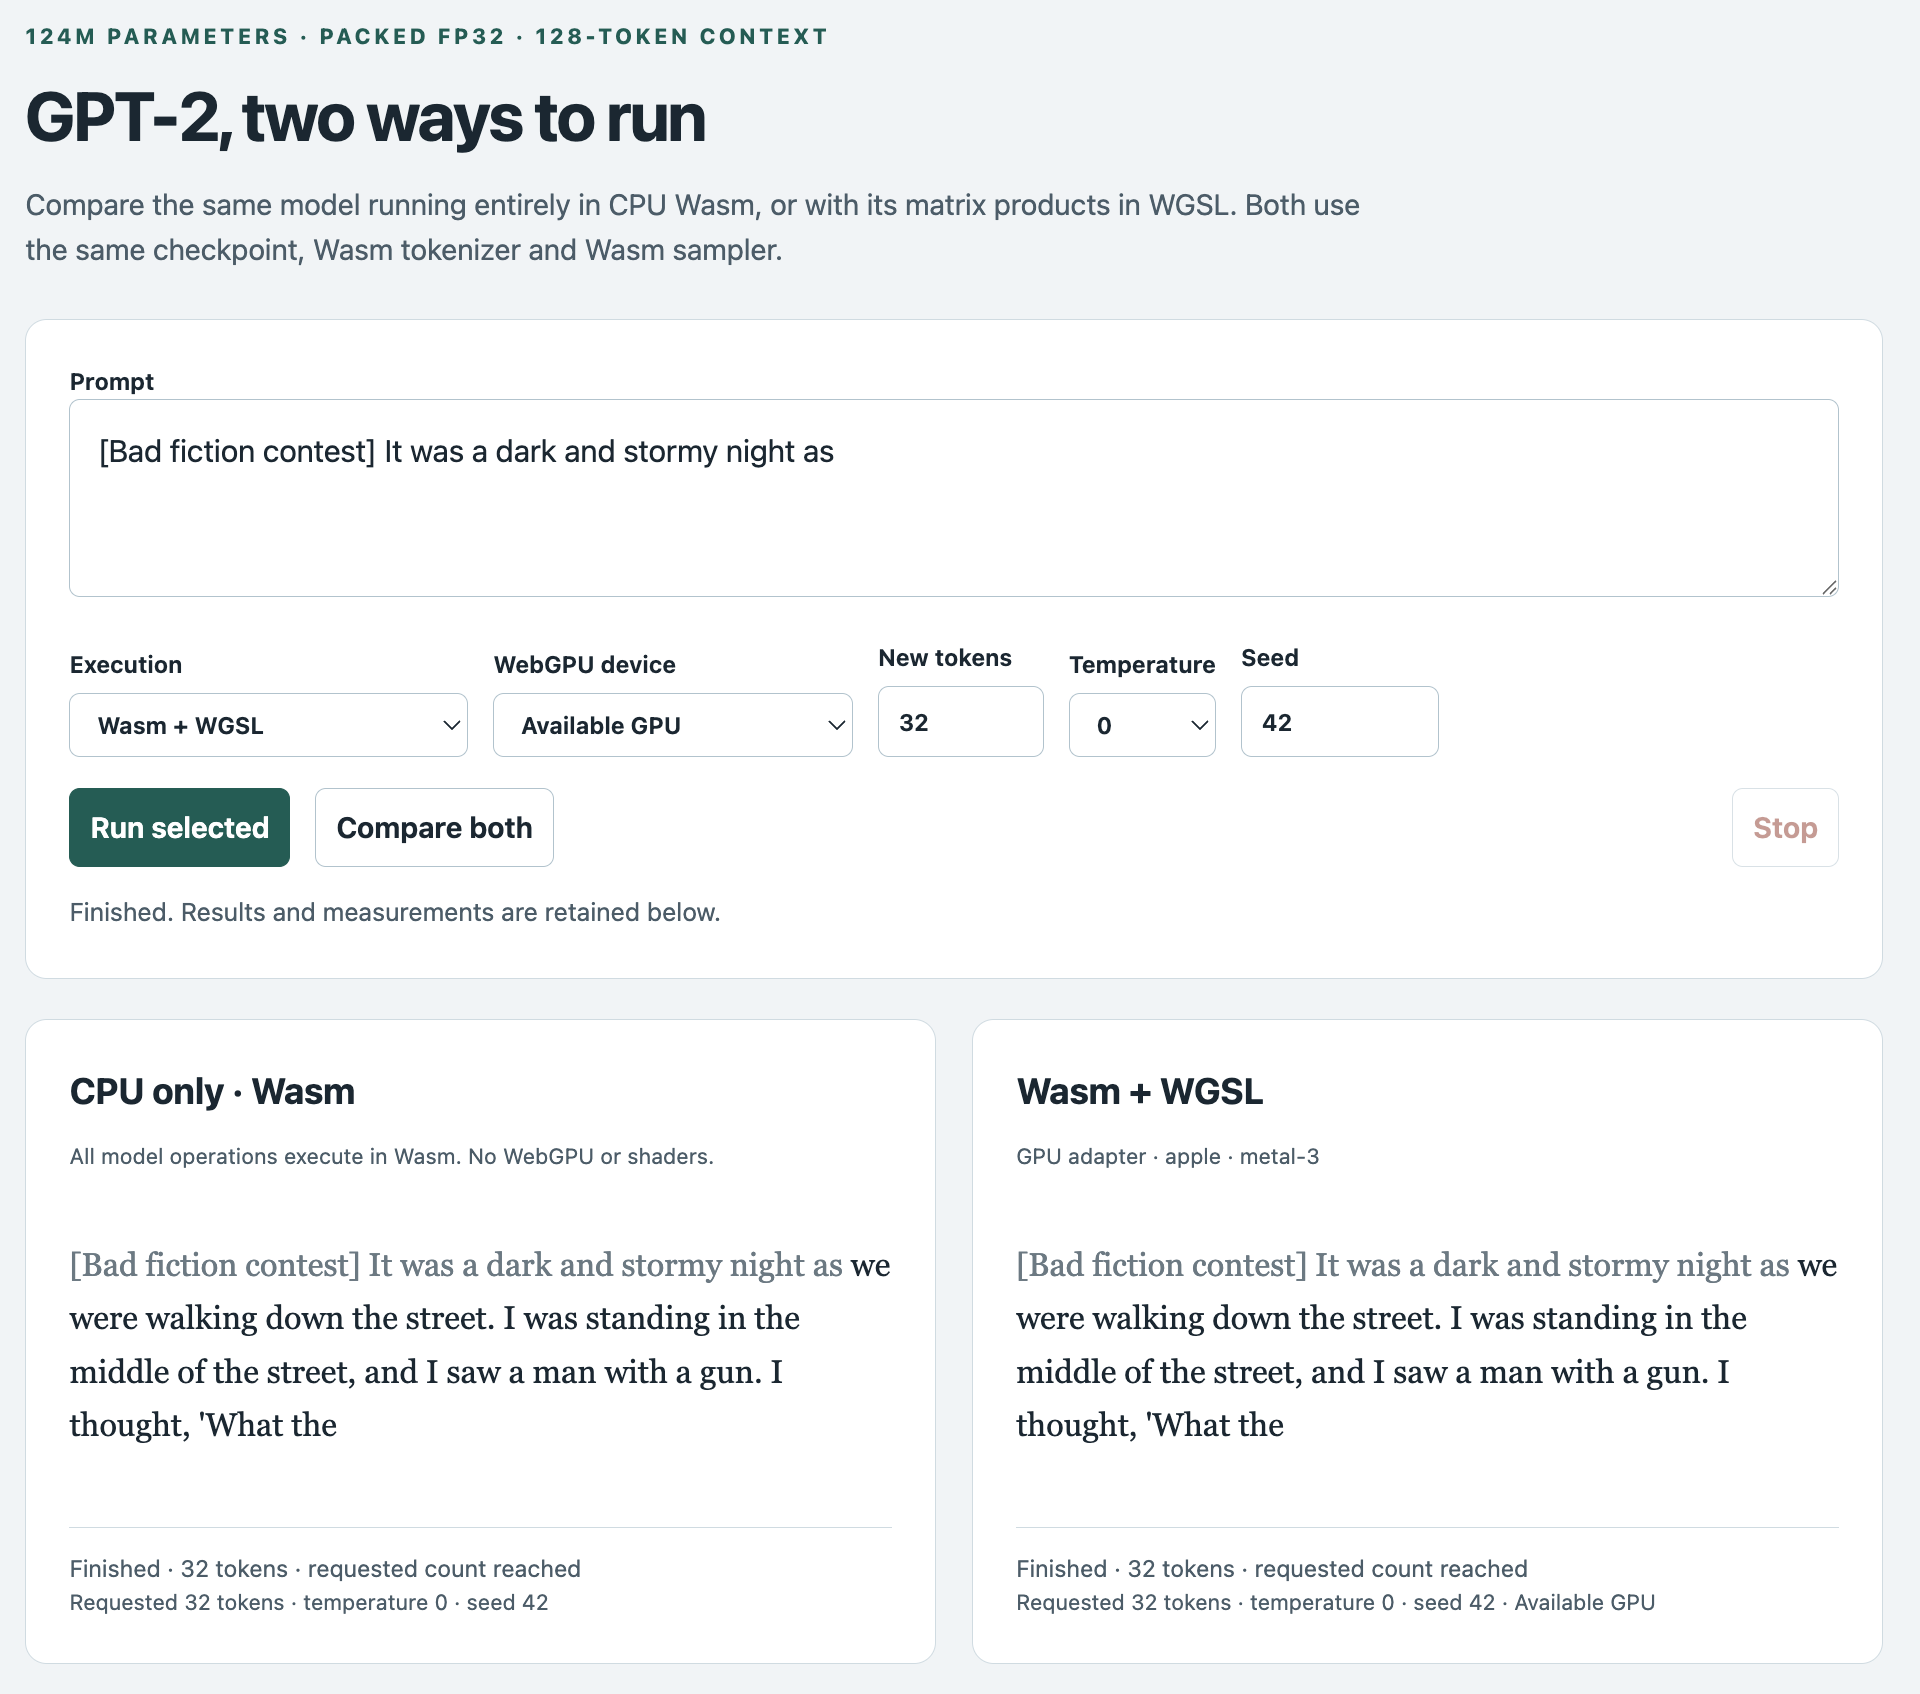
\includegraphics[width=\linewidth,height=0.85\textheight,keepaspectratio]{figures/gpt-1.png}
\caption{User-supplied browser completion comparison.  CPU WebAssembly and the hybrid Wasm/WGSL path show the same 32-token greedy continuation.  Settings, adapter labels, completion text, and stopping status remain visible.  The original image is included without content edits.}
\label{fig:browser-completion}
\end{figure}

\subsection{Timing definitions and the second image}

Figure~\ref{fig:browser-measurements} reproduces \code{gpt-2.png} from the same reported demonstration.  It records fourteen prompt tokens, thirty-two generated tokens, and thirty-one subsequent decode model steps for each backend.  The first generated token uses the logits produced by the final prompt call.  Each later generated token requires another model call.  Consequently, the decode-throughput numerator is 31 in this run~\cite{screenshots,browser-source}.

Prefill processes prompt tokens one at a time.  The reported prefill rate divides the number of completed prompt tokens by time spent in those model calls.  CPU WebAssembly takes 5.533 seconds at a displayed 2.53 tokens/s.  The hybrid takes 0.545 seconds at 25.71 tokens/s.  The corresponding elapsed-time ratio is approximately 10.15 using the displayed rounded durations.  The model-call timing includes host transfer and waiting time for WGSL.  Lazy creation and upload of weight views occur during prefill~\cite{screenshots,browser-source}.

Decode takes 11.820 seconds on CPU WebAssembly and 0.752 seconds on the hybrid path.  The displayed rates are 2.62 and 41.23 model steps/s.  The page reports a 15.72-fold ratio from its measurements.  Ratios recomputed from the rounded durations or rounded rates can differ in the last displayed digits.  These values describe the observed continuation and this implementation's timing definitions~\cite{screenshots}.

Setup takes 0.269 and 0.253 seconds.  The host measures setup from the start of a run through device and pipeline preparation, module and asset loading, tokenization, and worker readiness as applicable to the backend.  The first-token metric then begins after setup and ends at the worker's first token emission.  The displayed first-token times are 5.535 and 0.546 seconds.  Total elapsed time includes setup and is 17.647 seconds for CPU WebAssembly and 1.567 seconds for the hybrid path, a ratio of approximately 11.26 from the displayed numbers~\cite{screenshots,browser-source}.

Sampling and text-decoding counters have their own timed regions.  The image reports sampling times of 0.008 and 0.006 seconds and text-decoding times of 0.016 and 0.011 seconds.  The generation-elapsed measurement also contains loop, messaging, and other intervening work.  The backend comparison therefore supports a statement about complete generation and model-call throughput in addition to the selected kernel implementation~\cite{screenshots,browser-source}.

\begin{figure}[p]
\centering
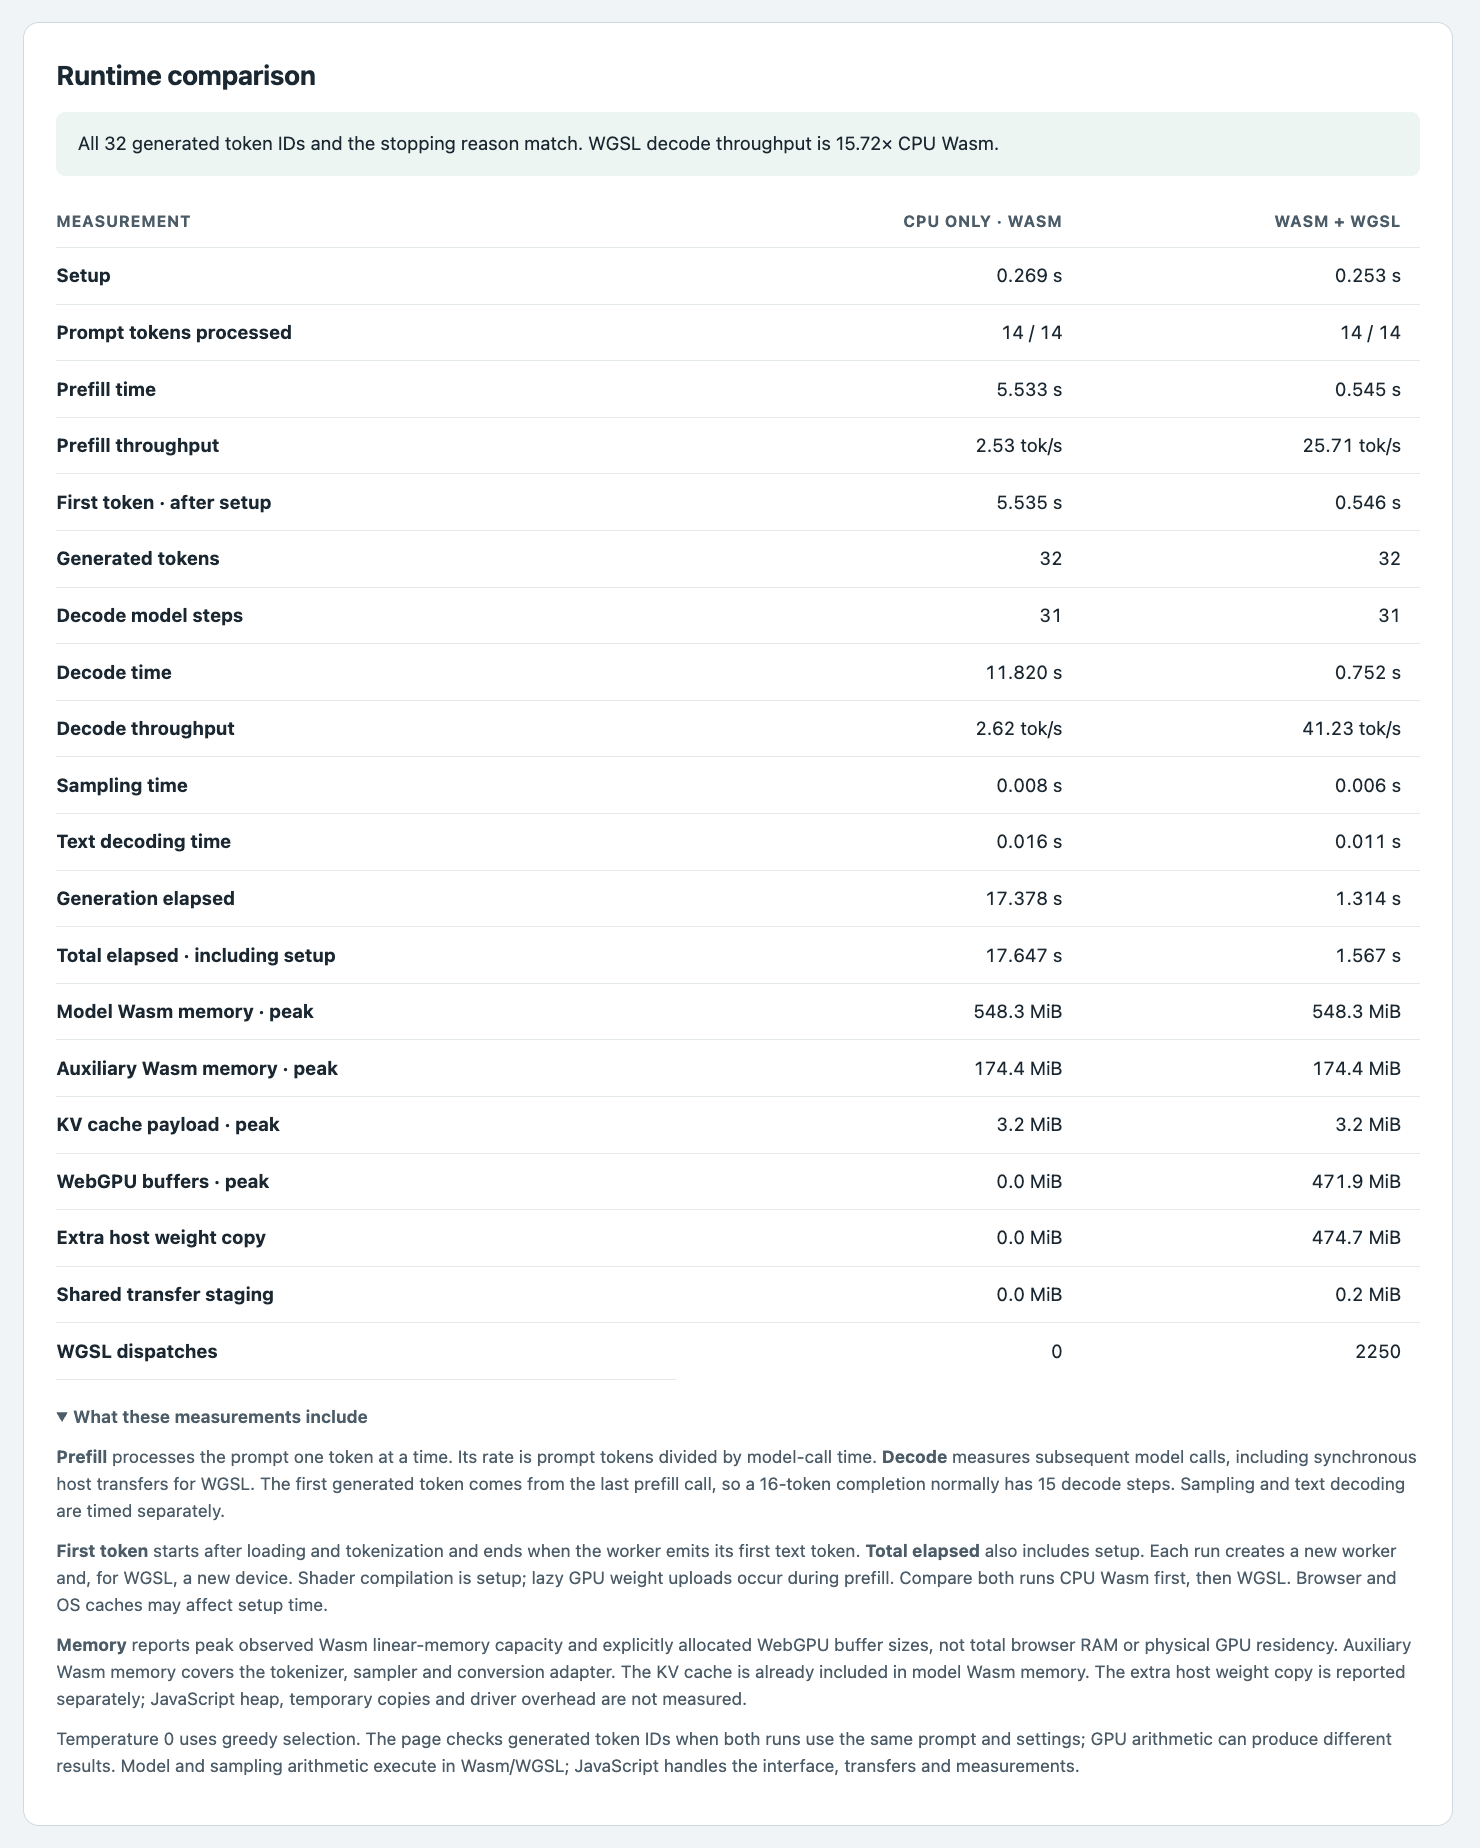
\includegraphics[width=\linewidth,height=0.87\textheight,keepaspectratio]{figures/gpt-2.png}
\caption{User-supplied runtime comparison for the completion in Figure~\ref{fig:browser-completion}.  The page reports matching token IDs and stopping reason, a 15.72-fold decode-throughput ratio, and separate timing, memory-capacity, and dispatch counters.  The explanatory text at the bottom defines the measurements.  The original image is included without content edits.}
\label{fig:browser-measurements}
\end{figure}

\subsection{Memory accounting and dispatch count}

The image reports peak model Wasm linear-memory capacity of 548.3 MiB for both paths and auxiliary Wasm capacity of 174.4 MiB.  The auxiliary total covers the tokenizer, sampler, and conversion adapter.  The 3.2 MiB peak key/value payload occupies part of the model memory.  Adding it again to model capacity would double-count those bytes.  These counters describe represented buffer capacities at observed points in the run~\cite{screenshots,browser-source}.

The hybrid path also reports 471.9 MiB of allocated WebGPU buffers, a 474.7 MiB host weight copy, and 0.2 MiB of shared staging.  The host weight-copy size follows from the 497,759,232-byte checkpoint.  The device buffers contain selected matrix views and transfer buffers.  The two paths can therefore have equal model linear-memory capacities while retaining different additional memory.  Physical GPU residency, JavaScript heap usage, temporary upload copies, browser internals, and driver allocations require other measurements~\cite{screenshots,browser-source}.

The dispatch count has a direct explanation in the source.  Four matrix shaders run per transformer layer and two shaders cover the vocabulary projection, giving
\[
12\times4+2=50
\]
dispatches per model call.  This run makes fourteen prefill calls and thirty-one decode calls, giving
\[
(14+31)\times50=2250.
\]
That value equals the image's reported dispatch count.  The cache payload after forty-five calls has $45\times73{,}728=3{,}317{,}760$ bytes, which rounds to the displayed 3.2 MiB.  These consistency checks relate the UI counters to the implemented call structure~\cite{screenshots,browser-source}.

\subsection{Experimental interpretation and provenance}

The screenshots provide a user-recorded browser completion and timing observation.  The retained evidence consists of the two original PNG files, their hashes, the visible settings and results, the user's environment description, and the inspected measurement source at the WGSL checkpoint.  The user identifies the browser as Chrome and the machine as a Mac mini with a 10-core CPU, a 10-core GPU, 32 GB of memory, 1 TB of storage, and Gigabit Ethernet.  The images contain the Apple/Metal adapter labels.  The Chrome version, chip model, and identity of the executed bundle remain unrecorded.  The report attributes the run and machine description to the user and the timing definitions to the inspected source~\cite{screenshots,browser-source}.

The fixed run order gives the second backend a different cache history.  Each run creates a fresh worker and, for WGSL, a fresh device, but browser and operating-system asset caches can persist between runs.  Pipeline preparation and weight upload also occur in different timed regions.  The displayed decode comparison includes the hybrid's synchronous transfer and wait costs, which makes it useful as a measurement of this complete model-call path.  Repeated trials with recorded versions and varied order would be needed to characterize variability or a wider hardware population~\cite{browser-source}.

The browser run extends the earlier report's execution evidence.  At the pinned branch checkpoint, the development journal still records browser execution as pending after automation failures.  It separately records a Node execution of the real CPU worker, matching sixteen selected tokens and 804,112 logit words against a native trace, plus cancellation and cleanup checks.  Those worker tests and the supplied browser images have different provenance.  This report retains both and identifies the screenshots as the new browser observation~\cite{wg-journal,browser-tests,screenshots}.

The browser CPU engine also differs from the Wasmtime configuration used by the native theorem application.  The strict formal arithmetic includes a selected arithmetic NaN word.  Applying that exact raw-word guarantee to browser WebAssembly requires evidence for the browser's arithmetic behavior on the relevant domain.  The hybrid adds the shader arithmetic and transfer premises described in Section~\ref{sec:hybrid}.  Matching text and token IDs in the displayed run supports that run's observed behavior.  Establishing those premises for every permitted weight array requires a stronger runtime correspondence result.

\section{Related work and literature-search assessment}
\label{sec:related}

\subsection{Search scope and comparison criteria}

The literature search took place on 19 September 2026.  It covered papers, technical reports, and public repositories concerning formal verification of transformer inference, executable neural networks, verified numerical software, compiler correctness, and cryptographic proofs of language-model evaluation.  Search terms combined GPT-2, transformer, and LLM inference with formal verification, executable, binary, Lean, Coq/Rocq, Isabelle, CompCert, CakeML, and verified compilation.  Follow-up searches and source inspection examined the strongest candidate claims.  The assessment uses primary papers and project sources~\cite{lit-torchlean,lit-hls,lit-gross,lit-rush,lit-somani,lit-zkllm,lit-zkgpt,lit-deepprove,lit-laproof}.

Five questions determine comparability with the present result.  First, what object does the theorem describe: a mathematical network, a source program, an intermediate representation, a shader, a binary, or one execution trace?  Second, what arithmetic does it specify: real, rational, quantized integer, finite-field, or floating-point computation?  Third, which inputs and weights does it quantify over?  Fourth, which translation and execution components remain assumptions?  Fifth, how is the proof checked and associated with the deployed program?  These questions expose differences that a shared use of the word ``verified'' can conceal.

A correctness theorem for the present CPU artifact has the schematic form
\[
\forall W,T.\quad \operatorname{Valid}(W,T)
\Longrightarrow
\operatorname{Exec}(B,W,T)=\operatorname{Source}(W,T),
\]
with successful termination and byte observations represented by the session predicate.  Here $B$ is a fixed executable byte sequence.  A cryptographic inference certificate instead proves an encoded relation for supplied commitments, an input, and an output, subject to the proof system's soundness assumptions.  A robustness theorem can quantify over many perturbed inputs while targeting an output property.  These are distinct propositions with different applications.

The search inspected stated theorem boundaries and selected definitions.  Independent proof rebuilding and full dependency audits remain outside this source review.  Repository pages describe development snapshots and can change after the search date.  Table~\ref{tab:related} records the comparison at the inspected versions.

\begin{longtable}{L{0.20\linewidth}L{0.34\linewidth}L{0.37\linewidth}}
\caption{Closest related results and their proof subjects.}\label{tab:related}\\
\toprule
Work & Established or reported result & Relation to the present proof\\
\midrule
\endfirsthead
\toprule Work & Established or reported result & Relation to the present proof\\\midrule
\endhead
TorchLean~\cite{lit-torchlean} & Lean network semantics, FP32 models, and source-to-IR correctness for a forward subset. & Shares source semantics and arithmetic concerns.  Target-runtime correspondence is future work.\\
HLS transformation verification~\cite{lit-hls} & Equivalence of C/C++ implementations, including a complete optimized BERT layer. & Shares implementation-equivalence goals.  The checked boundary ends before hardware synthesis.\\
Gross et al.~\cite{lit-gross} & Accuracy lower bounds for small trained Max-of-$K$ transformers. & Proves model behavior.  Floating-point correspondence is a separate future obligation.\\
Lean Verified Transformers~\cite{lit-rush} & Rational-arithmetic invariants and equivalence of transformer formulations. & Provides algebraic source-level results for simplified operations.\\
Verifiable Transformers~\cite{lit-somani} & SMT task-property proofs for a modified GPT-2-scale model on a fixed prompt domain. & Targets task decisions on a finite domain with changed numerical and architectural components.\\
zkLLM and zkGPT~\cite{lit-zkllm,lit-zkgpt} & Cryptographic certificates for complete LLM inference evaluations. & Prove encoded execution relations per evaluation, using quantized arithmetic and cryptographic soundness.\\
DeepProve~\cite{lit-deepprove} & Implemented complete-model proof generation, including GPT-2. & Supplies a current quantized-inference proving system.\\
LAProof~\cite{lit-laproof} & Coq numerical error proofs connected to a C sparse matrix-vector implementation. & Establishes a precedent for composing floating-point mathematics and low-level program proofs.\\
\bottomrule
\end{longtable}

\subsection{TorchLean and executable network semantics}

TorchLean formalizes neural-network semantics in Lean, with an operator-tagged graph representation, a PyTorch-like model interface, executable arithmetic, and verification machinery.  Its forward-compilation theorem covers a first-order subset and relates source evaluation to graph evaluation.  Its FP32 account distinguishes executable bit-level arithmetic from real-valued rounded models.  Attention and GPT-style examples make it the closest inspected proof-assistant infrastructure to the present inference work~\cite{lit-torchlean}.

The paper's Appendix D.1 identifies target-runtime correspondence as future work.  It requires a fixed arithmetic configuration, including denormal handling, reassociation, fusion, and reduction order, plus a relation between compiled runtime outputs and the selected executable model.  That boundary is decisive for this comparison.  LeanExe's CPU artifact proof covers the emitted WebAssembly instruction and memory computation under Talos semantics.  Its native application still trusts Wasmtime and the host.  The WGSL result states the corresponding external-execution requirement as a theorem premise.  TorchLean and LeanExe thus address related semantic layers with different completed target connections~\cite{lit-torchlean}.

\subsection{Verification of optimized transformer implementations}

Pouchet and coauthors verify equivalence between C/C++ functions used as inputs to high-level synthesis.  Their analysis handles statically interpretable control flow and transformations involving loops, buffers, layouts, and FIFO communication.  The FPGA 2024 evaluation includes a complete BERT layer with twelve attention heads, feature dimension 768, and feed-forward dimension 3072.  The paper states that correctness of the subsequent HLS backend is assumed~\cite{lit-hls}.

This work establishes a close implementation-level precedent.  Its comparison concerns two concrete algorithm implementations and complex storage transformations.  The target boundary and demonstrated model extent distinguish it from the GPT-2 artifact result: C/C++ source precedes hardware synthesis, and the transformer example covers one layer.  The WGSL packed-layout proofs solve a related correspondence problem between tensor views and matrix operations, then use replacement-call postconditions in a full cached controller.  The CPU binary result adds a checked decoding and translation connection to the executable module~\cite{lit-hls}.

\subsection{Properties of trained and algebraic transformer models}

Gross and coauthors derive computer-assisted accuracy lower bounds for small transformers trained on Max-of-$K$.  Their NeurIPS 2024 work studies proof strategies and the relation between mechanistic understanding and compact performance guarantees.  Its Appendix A.7 describes the additional error arguments needed to connect real-number reasoning and floating-point evaluation, and leaves that connection to future work~\cite{lit-gross}.

Their theorem objective concerns what a trained network predicts.  The present source-agreement theorem concerns how an executable realizes a specified computation.  The two kinds of result could compose if a behavioral theorem used the same source semantics, weight values, and input domain.  For example, a proved property of \code{cachedStep}'s logit vector could transfer through its exact artifact execution theorem to the represented output bytes.  That composition would require proving the source property and satisfying its hypotheses in addition to the execution result.

Rush's Lean Verified Transformers development proves invariants and equivalences associated with batching, parallelism, tiled attention, and state-space formulations.  The inspected source represents values by rationals.  Its \code{softmax\_like} definition uses normalized $1+\operatorname{relu}$ weights, and its tiled-attention proof preserves that selected definition.  The file supplies checked source-level algebraic arguments~\cite{lit-rush}.

Algebraic transformations have a separate floating-point obligation when operation order changes.  The present strict dot-product specification resolves that obligation by preserving ordered, separately rounded multiplication and addition.  Parallel execution distributes output coordinates while retaining each coordinate's reduction order.  An optimization that reorders or fuses the reduction would need a different equality or an explicitly numerical relation.  This follows from the specified algorithm and determines which transformations the current exact theorem supports.

The Rocq Transformer repository supplies another source-level comparison.  It encodes transformer architecture through dependent tensor shapes and gives structural properties.  Its documentation distinguishes implemented structural operations from numerical operations represented by parameters, including matrix multiplication.  Its established boundary is therefore shape and architecture reasoning with abstract numerical components~\cite{lit-rocq}.  Connecting such a model to an executable would require implementations of those components and proofs relating the chosen numerical behavior to them.

\subsection{SMT properties for a modified GPT-2-scale model}

Somani's Verifiable Transformers repository reports SMT proofs for a quote-closing task on a fixed 1,280-prompt domain.  The described model uses a GPT-2-scale base modified for the verification method: normalization is removed, GELU is replaced by LeakyReLU, and the task circuit uses synthesized symbolic attention.  The verified decision compares task candidates.  The repository separates this result from another task for which full verification remained unattempted at inspection~\cite{lit-somani}.

The property, data domain, and modified model define the result's scope.  LeanExe's theorem instead fixes the cached FP32 algorithm and proves all its output bytes for arbitrary runtime weight values and valid token lists.  Task accuracy and implementation equality establish different propositions.  Both the property and the quantified domain determine comparability~\cite{lit-somani}.

\subsection{Cryptographic proofs of complete inference}

zkLLM provides zero-knowledge proofs for language-model inference using tensor-oriented protocols, including attention and lookup arguments.  Its soundness account uses cryptographic commitments and randomized algebraic checks.  The paper states the negligible-error conditions and describes numerical tolerances arising from quantization and attention approximation.  Its evaluation covers models up to thirteen billion parameters~\cite{lit-zkllm}.

zkGPT implements a non-interactive proof system for GPT-2 inference.  Its arithmetic relations cover linear and nonlinear layers, and its implementation optimizes their proof cost.  Section 9.3 identifies dependence on quantization as the reason its current construction cannot directly certify floating-point inference.  The paper and artifact provide prior evidence that complete GPT-style model evaluation can produce a checkable cryptographic certificate~\cite{lit-zkgpt}.

DeepProve is a further implemented system in this category.  Its repository documents complete GPT-2, Gemma, and Llama inference proofs, model loading, quantized execution, and proof/verification commands.  The described computation uses calibrated integer arithmetic, with a default 12-bit quantization setting, and proves the computation from embeddings through output selection using its cryptographic protocols~\cite{lit-deepprove}.

These results determine the scope of a priority claim.  Complete inference certificates existed before this report.  A certificate for an evaluation supplies evidence that its encoded input/output relation holds under the proof system's soundness assumptions.  A static program-correctness theorem supplies a reusable result for every input in its domain.  It can cover termination, memory behavior, and correspondence to a particular executable.  A system could combine both approaches: an implementation theorem could justify a proof-producing inference program, while runtime certificates could attest to remote evaluations.  Each layer would retain its own assumptions.

For the present work, the relevant distinction is the proof-assistant-checked relation between an executable inference module and its source recurrence.  A thirteen-billion-parameter cryptographic example can exceed GPT-2 in scale while proving a different proposition.  Likewise, a small source-level formalization can use a proof assistant while leaving compilation and storage implementation to separate work.  The comparison therefore uses the proof subject, arithmetic, quantification, and trusted execution components together.

\subsection{Verified floating-point numerical software}

LAProof provides Coq proofs for linear-algebra accuracy, including inner products, matrix-vector and matrix-matrix operations, and related additions.  It connects that mathematical development to a verified C sparse matrix-vector implementation using compressed sparse rows.  The proof accounts for representation and IEEE floating-point behavior, and the accuracy results include backward or mixed error bounds under their stated conditions~\cite{lit-laproof}.

This precedent shows that low-level numerical implementation proofs and floating-point analysis already have established techniques.  The GPT-2 contribution is their application and extension across a complete cached transformer, including the source-defined nonlinear routines and repeated session state.  The present exact theorem supplies equality with the Lean computation.  A later accuracy analysis could use the exact execution result to transfer a proved source-level bound to artifact outputs.  That would require its own numerical hypotheses and a theorem for the chosen source algorithm.

\subsection{Priority assessment}

The search found no earlier result establishing the same complete binary-to-source guarantee for GPT-style inference.  The supported claim is: to our knowledge, this development is the first proof-assistant-checked functional-correctness verification connecting a complete executable GPT-style inference module to its source algorithm, demonstrated for GPT-2 124M with a 128-token context.  The CPU result includes the frozen WebAssembly bytes and exact cache and logit observations for every permitted session.  This claim remains qualified by the search method and inspection depth stated above.

The WGSL contribution has its own scope: checked compilation of supported kernel definitions, exact packed-result correspondence, and reuse of the controller proof under an explicit host-execution premise.  Its theorem is conditional on strict shader behavior and transfers.  The supplied browser observation establishes a concrete successful comparison and its recorded timings.  The priority assessment for the CPU artifact proof therefore remains separate from any claim about universal correctness of browser or GPU execution.

\section{Assurance, review evidence, and remaining obligations}
\label{sec:assurance}

\subsection{Logical dependencies and deployment premises}

The proof assistant checks a proposition about specified semantics.  Applying that result to a deployed program requires an association with the executed bytes and an interpretation of the runtime as implementing those semantics.  Table~\ref{tab:assurance} identifies these layers for the two paths.  It also distinguishes assumptions expressed in theorem types from software components trusted when using the theorem on a physical machine.

\begin{longtable}{L{0.20\linewidth}L{0.34\linewidth}L{0.37\linewidth}}
\caption{Verification status by semantic boundary.}\label{tab:assurance}\\
\toprule
Boundary & CPU WebAssembly path & Hybrid Wasm/WGSL path\\
\midrule
\endfirsthead
\toprule Boundary & CPU WebAssembly path & Hybrid Wasm/WGSL path\\\midrule
\endhead
Source algorithm & Lean cached-step recurrence with fixed FP32 order. & The same recurrence, reached through checked matrix replacement equalities.\\
Scalar computation & All-word source/Talos equalities for the arithmetic used by GPT-2. & The same Wasm arithmetic plus strict shader addition and multiplication semantics.\\
Memory and session & Checked allocation, ownership, release, and 128-token composition. & Controller composition checked under external-call postconditions.\\
Executable identity & Frozen binary decoding, validation, and Talos-module equality. & Parsed hybrid module declarations and certified shader strings.  Hybrid binary certification remains an obligation.\\
External calls & The checked inference module has no imports. & \code{PackedBackend.Host} requires completed shader execution, exact transfers, and store preservation.\\
Physical execution & Wasmtime canonical-NaN mode and native host are trusted. & Native/browser hosts, WebGPU implementation, and strict arithmetic conformance are external premises.\\
Text interface & Host tokenization, sampling, and decoding surround the proved token/logit interface. & Wasm tokenizer, sampler, and conversion adapter surround the same inference interface.\\
Current run evidence & Recorded canonical-mode and PyTorch comparisons. & Recorded native CPU WebGPU comparisons and supplied browser images.\\
\bottomrule
\end{longtable}

The final CPU artifact theorem uses the three standard logical axioms listed in Section~\ref{sec:boundary}.  The hybrid theorem's recorded audits use the same allowance.  A host-execution hypothesis can appear as an ordinary parameter without adding an axiom declaration.  Auditing both the theorem type and its transitive axiom dependencies is therefore necessary to state the result's meaning~\cite{review,wg-composition,wg-backend}.

The memory-capacity assumptions also require a deployment interpretation.  The formal session derives sufficient modeled capacity through the supported length.  Native process limits, browser memory restrictions, external GPU allocation, and device loss can affect a physical run.  A proof of successful execution in the formal store model supplies its stated semantics under that model's allocation behavior.  Deployments need resources that realize those premises~\cite{budget,wg-host}.

\subsection{Evidence retained from proof review}

The CPU report retains a successful source-driven regeneration and proof check, a focused exact-artifact check, and a separate statement review with seven accepted corollaries and the combined theorem's axiom report.  Source-identity records cover the cited proof and implementation files.  The review also compared the built command-line binary with the frozen artifact byte for byte.  These records support the stated checkpoint result~\cite{cpu-report-evidence}.

The WGSL report retains focused compiler and statement-proof checks from an isolated checkout.  Source equality, static validity, invocation correctness, and shared index and dispatch-geometry theorem audits passed for the split review examples.  The full extracted certificate corpus timed out after 90 seconds on its first positive shader under the one-core resource limit.  A separate token-parser certificate passed, while a lexical certificate exceeded 60 seconds.  The failed attempts remain in the review record and identify a certificate-checking cost that affected reproduction~\cite{wg-review}.

The complete hybrid session result and full-model native comparison come from the branch's integration journal and generation code.  The earlier review inspected those sources and their public theorem requirements.  Full hybrid session and checkpoint reproduction remained pending in that review.  Their generated proof objects and runtime reports reside in ignored build directories.  The current report attributes those outcomes to the recorded integration runs~\cite{wg-journal,wg-review}.

The browser comparison adds user-supplied execution evidence after that review.  Its two source commits extend the host and interface while retaining the inference and shader proof sources.  This report checks the measurement definitions and numerical consistency of the displayed counters.  Its document build and review produce a new report, while the proof and execution records retain the dates and environments in which they were obtained~\cite{browser-source,browser-tests,screenshots}.

\subsection{Runtime arithmetic and exact results}

The CPU exact-result theorem uses one selected word semantics.  The Wasmtime host configures arithmetic NaN canonicalization to support that interpretation.  The WGSL strict semantics also preserves separate multiplication and addition, source reduction order, represented subnormals, and specified exceptional results.  WebGPU implementations have permitted choices that can differ from those conditions.  A successful shader compile establishes acceptance of the program by the implementation, while a runtime correspondence result would establish the required behavior~\cite{wasmtime,wg-wgsl,wg-execution}.

An implementation can produce the same selected token while differing in logit words.  Greedy decoding depends on the largest component and its tie-breaking rule.  Small changes to lower-ranked values can leave the selected token unchanged.  Conversely, a small difference near an argmax tie can change the next token and every subsequent input.  The screenshot comparison therefore records token-sequence agreement.  The native word-comparison tests examine a stronger equality on their tested inputs~\cite{wg-tests,screenshots}.

Future arithmetic work has two distinct targets.  A strict backend could establish or enforce the word semantics used by the existing equality theorem.  A numerical refinement could admit specified fusion, rounding, or approximation behavior and prove a bound relative to the source.  The latter would need explicit domain and stability conditions that keep the bound meaningful through normalization, softmax, and repeated transformer blocks.  The present hybrid theorem retains the strict semantics and states its external execution requirement.

\subsection{Artifact packaging and repeatable checking}

The CPU CLI currently compiles the source it finds and runs that output.  The reviewed output matched the registered artifact.  Preserving the same assurance after source or compiler changes requires another identity check or a new artifact proof.  An integrated CLI check against the proved bytes would make that association part of every run.  The combined GPT-2 artifact theorem's strict three-axiom audit also remains a separate review step rather than the generic package policy used for other artifacts~\cite{driver,artifactgate,review}.

The hybrid source-build gate checks the parent, produces the modified controller and six shaders, checks replacement and composition proofs, and copies files into a bundle.  Later native and browser execution reads those bundle files.  A runtime identity gate would bind the loaded files to the checked strings and module.  Extending binary decoding and translation proofs to the hybrid bytes would close the external-parser boundary.  These are identifiable obligations at the executable-association layer~\cite{wg-build,wg-host}.

Portable retention of generated hybrid certificates and machine-readable execution records would improve independent reproduction.  A source revision and a journal describe the construction, while a preserved checked package allows a reviewer to inspect the exact generated theorem types and inputs without repeating every production step.  The existing CPU artifact package demonstrates that form of association.  The shader compiler already emits declarations intended for separate checking~\cite{artifact,wg-compiler,wg-review}.

\subsection{Extensions supported by the present proof structure}

A larger context changes the cache bound, loop ranges, and session allocation estimate.  A larger architecture changes dimensions, tensor offsets, and the traversal count.  The generic arithmetic and memory lemmas can remain applicable, while concrete loops, generated instruction equalities, and resource calculations need new instances or proofs.  The current result fixes those quantities for GPT-2/128 and quantifies over the data within them~\cite{session,budget}.

An alternative cache layout or a fused kernel would change a proof interface.  The layout relation must identify the new memory representation with source values.  A fused numerical operation must satisfy the arithmetic relation selected by the caller.  The hybrid development illustrates this method for matrix replacement: first establish the new computation and representation result, then prove that its call supplies the old controller's required postcondition.  That decomposition permits reuse where the interface remains valid~\cite{wg-packedsource,wg-backend,wg-transport}.

A proof of equality between cached inference and a separate full-prefix algorithm would establish another algorithmic relation.  The present recurrence is the source specification, and the recorded short-prefix comparison is a test between implementations.  A full-prefix equivalence theorem would need to account for operation ordering, cache content, and the chosen numerical routines.  A theorem about language quality or model behavior would add another property of that source computation.  These extensions have explicit proof targets beyond the completed execution result~\cite{cached,testcode}.

\section{Conclusion}

The development connects a complete GPT-2 cached-inference algorithm in Lean to a frozen WebAssembly binary, with checked termination, exact output bytes, and the memory behavior required across a 128-token session.  Integer-defined floating-point semantics, packed-memory relations, loop invariants, ownership proofs, and whole-module translation equality supply the connection.  Runtime weights remain quantified data, so changing their values within the fixed representation preserves the execution theorem.

The WGSL extension proves selected shader programs implement their Lean kernel definitions and that the packed results equal the matrix operations used by the controller.  Reused helper proofs and rechecked controller composition establish the complete hybrid recurrence under explicit external-execution and transfer premises.  Native comparisons and the supplied browser run document successful executions within the tested conditions.  The browser images record matching 32-token completions and their timing and memory counters.  The literature comparison places these results alongside source-level transformer proofs, implementation-equivalence checks, and cryptographic inference certificates, with the proof subject and assumptions stated for each.

\appendix
\section{Theorem and source reference}
\label{sec:reference}

\subsection{Public declarations and inspection order}

The CPU artifact declaration provides the narrowest entry point for inspecting the complete executable claim.  Its conclusion names decoding, validation, and the module-parameterized session specification.  Following that specification reveals the initialization sequence and \code{Session.RunsFor}.  The source trace then identifies the exact Lean function whose cache and logits the session observes.  The component entry proof supplies the lower-level output and heap facts~\cite{artifact,session,entry}.

\begin{longtable}{L{0.41\linewidth}L{0.50\linewidth}}
\caption{Selected declarations and their roles.}\\
\toprule
Declaration & Role\\
\midrule
\endfirsthead
\toprule Declaration & Role\\\midrule
\endhead
\longcode{LeanExe.Models.Gpt2.cachedStep} & Source algorithm for one accepted or rejected token call.\\
\longcode{Project.Gpt2CachedStep.Spec.cachedStep\_exact} & Successful target entry with source cache/logit bytes and heap preservation under represented-input and resource premises.\\
\longcode{Project.Gpt2CachedStep.Session.Ready} & Heap, ownership, cache size, separation, and allocation invariant.\\
\longcode{Project.Gpt2CachedStep.Session.RunsFor} & Observable sequence of calls, byte reads, and releases for a module parameter.\\
\longcode{Project.Gpt2CachedStep.Spec.gpt2\_128\_exact} & Initialization and complete source-trace agreement for valid token lists.\\
\longcode{Project.Gpt2CachedStep.Spec.ExactSpecFor} & Module-parameterized form used to transfer the result through decoded-module equality.\\
\longcode{Project.Gpt2CachedStep.Artifact.artifact\_gpt2\_128\_exact} & Combined frozen-binary decode, validation, and session theorem.\\
\longcode{LeanExe.WGSL.Statement.Implements} & Successful invocation result for a shader string under the supported statement semantics.\\
\longcode{Project.Gpt2.PackedBackend.Kernels} & Six shader texts together with their checked invocation results.\\
\longcode{Project.Gpt2.PackedBackend.Code} & Imported and defined function identities in the hybrid module.\\
\longcode{Project.Gpt2.PackedBackend.Host} & External-call execution, output transfer, and store-preservation premise.\\
\longcode{Project.Gpt2Hybrid.Spec.gpt2\_128\_exact} & Generated conditional complete-session theorem for the hybrid controller.\\
\bottomrule
\end{longtable}

The CPU proof sources remain at the CPU checkpoint named in Section~\ref{sec:context}.  Shader, packed replacement, host, and browser references use the WGSL checkpoint.  This separation avoids assigning the CPU artifact's byte identity to a later imported-controller binary.  The companion evidence records the file identities used while preparing this report.

\subsection{Reproduction commands and their subjects}

The CPU command-line and focused artifact-check commands appear in Section~\ref{sec:tests}.  They distinguish model execution, source-driven proof regeneration, exact-file checking, and theorem-statement auditing.  Each command has a different subject.  A successful text completion exercises the host path.  A successful artifact check connects a file with the proved byte sequence and registered proof.  A theorem audit examines the selected declarations' logical dependencies~\cite{guide,artifactgate,reviewlemmas}.

The hybrid source-build and execution entry points at the WGSL checkpoint are
\begin{verbatim}
tools/gpt2-packed build build/gpt2/packed-new
tools/gpt2-packed --prompt 'The purpose of science is' \
  --generate 16 --temperature 0
tools/gpt2-packed serve 8080
\end{verbatim}
The build destination must be new.  The source-build tool uses the configured Python environment to prepare checkpoint assets and requires the pinned Lean, Wasm, Wasmtime, and native WebGPU dependencies.  Inference executes through the bundled Wasm and WGSL files.  The browser page is available at \code{http://127.0.0.1:8080}.  The bundle selection and supported generation settings are documented in the packed guide~\cite{wg-packedguide,wg-build}.

Every Lean or Lake command in the repository runs through \code{tools/leanrun}.  The runner serializes Lean work and applies the repository's resource limits in its standard mode.  Reproduction records need to include those limits because certificate checking can reach a timeout before yielding a proof result.  The retained WGSL lexical timeout is one example.  A successful cached check and a complete cold build also have different costs and should retain that distinction in their records~\cite{wg-review}.


\begin{thebibliography}{99}
\bibitem{repo} LeanExe repository.  Source checkpoint \longcode{4360920c3060d1c625b1860229b5116804d177c8}.  \url{https://github.com/jsmorph/leanexe/tree/4360920c3060d1c625b1860229b5116804d177c8}.
\bibitem{artifact} LeanExe.  \src{proofs/talos/lean/Project/Gpt2CachedStep/ArtifactBytes.lean}{Embedded GPT-2 binary}, \src{proofs/talos/lean/Project/Gpt2CachedStep/ArtifactDecode.lean}{complete decoding theorem}, \src{proofs/talos/lean/Project/Gpt2CachedStep/ArtifactValidation.lean}{validation theorem}, and \src{proofs/talos/lean/Project/Gpt2CachedStep/ArtifactTranslation.lean}{translation equality and combined execution theorem}.  Report checkpoint.
\bibitem{binary} LeanExe.  \src{proofs/talos/lean/Project/Artifact/Binary/Grammar.lean}{Binary grammar}, \src{proofs/talos/lean/Project/Artifact/Binary/Validity.lean}{validation rules}, \src{proofs/talos/lean/Project/Artifact/Binary/Proof/Decode.lean}{decoder soundness}, \src{proofs/talos/lean/Project/Artifact/Binary/Proof/Validate.lean}{validator soundness}, and \src{proofs/talos/lean/Project/Artifact/Binary/Translate.lean}{Talos translation}.  Report checkpoint.
\bibitem{artifactgate} LeanExe.  \src{tools/artifact-proof.js}{Exact-artifact checker and axiom policy} and \src{proofs/talos/lean/Project/Artifact/Binary/CheckFile.lean}{external-file comparison}.  Report checkpoint.
\bibitem{review} LeanExe.  \src{devnotes.md}{Development journal, entries for the completed artifact proof and the 19 September critical review}.  Report checkpoint.
\bibitem{reviewlemmas} LeanExe.  \src{proofs/talos/reviews/gpt2-2026-09-19.lean}{Checked review corollaries and final-theorem axiom audit}.  Report checkpoint.
\bibitem{leanaxioms} Lean contributors.  \emph{Logical axioms and native evaluation}.  Lean revision \longcode{6a10ac8c22beadecabdbb0919c2b50214762f91d}.  \url{https://github.com/leanprover/lean4/blob/6a10ac8c22beadecabdbb0919c2b50214762f91d/src/Init/Prelude.lean} and \url{https://github.com/leanprover/lean4/blob/6a10ac8c22beadecabdbb0919c2b50214762f91d/src/Init/Core.lean}.
\bibitem{session} LeanExe.  \src{proofs/talos/lean/Project/Gpt2CachedStep/Session/Spec.lean}{Session theorem} and \src{proofs/talos/lean/Project/Gpt2CachedStep/Session/State.lean}{source trace and invocation predicates}.  Report checkpoint.
\bibitem{subset} Codex GPT-6 and Jamie Stephens.  \emph{The LeanExe Subset: Types, Extraction, and Execution}.  marXiv:2609.00005v6, 2026.  \url{http://127.0.0.1:8405/abs/2609.00005v6}.
\bibitem{talos} Talos.  Lean WebAssembly execution and proof library.  Revision \longcode{87e3aa5e8f6e6f3b3eb5e7e4c5aba43071002d47}.  \url{https://github.com/jsmorph/talos/tree/87e3aa5e8f6e6f3b3eb5e7e4c5aba43071002d47}.
\bibitem{gpt2} OpenAI.  GPT-2 model source, including cached attention and tied output projection.  \url{https://github.com/openai/gpt-2/blob/master/src/model.py}.
\bibitem{manifest} LeanExe.  \src{data/gpt2-124m/manifest.json}{Pretrained checkpoint manifest}.  Report checkpoint.  Weights from \url{https://huggingface.co/openai-community/gpt2/tree/607a30d783dfa663caf39e06633721c8d4cfcd7e}.
\bibitem{cached} LeanExe.  \src{LeanExe/Models/Gpt2/Cached.lean}{Cached GPT-2 source} and \src{LeanExe/Models/Gpt2/Inference.lean}{model dimensions and vocabulary projection}.  Report checkpoint.
\bibitem{kernels} LeanExe.  \src{LeanExe/Models/Gpt2/Kernel.lean}{FP32 tensor kernels}.  Report checkpoint.
\bibitem{packed} LeanExe.  \src{LeanExe/Packed.lean}{Packed word operations} and \src{proofs/talos/lean/Project/ProofKit/PackedMemory.lean}{packed-memory proof definitions}.  Report checkpoint.
\bibitem{entry} LeanExe.  \src{proofs/talos/lean/Project/Gpt2CachedStep/Spec.lean}{Complete cached-step theorem and component imports}.  Report checkpoint.
\bibitem{initialize} LeanExe.  \src{proofs/talos/lean/Project/Gpt2CachedStep/Initialize.lean}{Module reset, allocation, input, and export identities}.  Report checkpoint.
\bibitem{numerics} LeanExe.  \src{LeanExe/Models/Gpt2/Numerics.lean}{Exponential, GELU, and word-comparison definitions}.  Report checkpoint.
\bibitem{termination} Talos.  \emph{Fuel-free specification predicates}.  \url{https://github.com/jsmorph/talos/blob/87e3aa5e8f6e6f3b3eb5e7e4c5aba43071002d47/interpreter/Interpreter/Wasm/Spec/Defs.lean}.
\bibitem{input} LeanExe.  \src{proofs/talos/lean/Project/ProofKit/PackedInput.lean}{Packed input encoding} and \src{proofs/talos/lean/Project/ProofKit/PackedAllocExport.lean}{exported allocation proof}.  Report checkpoint.
\bibitem{f32} LeanExe.  \src{proofs/talos/lean/Project/ProofKit/F32Source.lean}{Logical Float32 source correspondence}, with \src{proofs/talos/lean/Project/ProofKit/F32Add.lean}{addition}, \src{proofs/talos/lean/Project/ProofKit/F32Sub.lean}{subtraction}, \src{proofs/talos/lean/Project/ProofKit/F32Mul.lean}{multiplication}, \src{proofs/talos/lean/Project/ProofKit/F32Div.lean}{division}, and \src{proofs/talos/lean/Project/ProofKit/F32Sqrt.lean}{square-root equalities}.  Report checkpoint.
\bibitem{leanfloat} Lean contributors.  \emph{Float32 logical model}.  Lean revision \longcode{6a10ac8c22beadecabdbb0919c2b50214762f91d}.  \url{https://github.com/leanprover/lean4/blob/6a10ac8c22beadecabdbb0919c2b50214762f91d/src/Init/Data/Float/Model/Float32.lean}.
\bibitem{loops} LeanExe.  \src{proofs/talos/lean/Project/ProofKit/RangeFoldLoop.lean}{Range-fold loop proofs}.  Report checkpoint.
\bibitem{budget} LeanExe.  \src{proofs/talos/lean/Project/ProofKit/HeapGrowth.lean}{Heap growth} and \src{proofs/talos/lean/Project/Gpt2CachedStep/Entry/Budget.lean}{cached-step allocation budget}.  Report checkpoint.
\bibitem{gate} LeanExe.  \src{tools/talos-lib.js}{Source-driven generation and proof-check driver}.  Report checkpoint.
\bibitem{wasmspec} WebAssembly Community Group.  \emph{WebAssembly Specification: Numerics}.  \url{https://webassembly.github.io/spec/core/exec/numerics.html}.
\bibitem{wasmtime} Bytecode Alliance.  \emph{Wasmtime C API: NaN canonicalization configuration}.  \url{https://docs.wasmtime.dev/c-api/config_8h.html}.
\bibitem{driver} LeanExe.  \src{training/gpt2/wasm.py}{WASM command-line client}, \src{training/gpt2/reference.py}{CPU PyTorch reference}, and \src{tools/wasmtime-host.c}{Wasmtime host}.  Report checkpoint.
\bibitem{tests} LeanExe.  \src{data/gpt2-124m/canonical-mode-test.json}{Canonical-mode runtime test record}, 18 September 2026.  Report checkpoint.
\bibitem{testcode} LeanExe.  \src{training/gpt2/test_wasm.py}{128-position comparison test} and \src{test/packed.js}{packed execution and completion tests}.  Report checkpoint.
\bibitem{wasmtimeintro} Bytecode Alliance.  \emph{Wasmtime: Introduction}.  \url{https://docs.wasmtime.dev/introduction.html}.
\bibitem{talosbefore} Talos.  \emph{Floating-point evaluator before the integer-arithmetic extensions}.  Revision \longcode{fda69ca67a81ea4f1fa4e376bdc5861d9fe5479a}.  \url{https://github.com/jsmorph/talos/blob/fda69ca67a81ea4f1fa4e376bdc5861d9fe5479a/interpreter/Interpreter/Wasm/Float.lean}.
\bibitem{talosfp} Talos.  \talossrc{interpreter/Interpreter/Wasm/IEEE32.lean}{Integer-defined binary32 arithmetic} and \talossrc{interpreter/Interpreter/Wasm/IEEE64.lean}{binary64 arithmetic}.  Pinned Talos revision.
\bibitem{talosdispatch} Talos.  \talossrc{interpreter/Interpreter/Wasm/Float.lean}{Floating-point operation dispatch}, \talossrc{interpreter/Interpreter/Wasm/Semantics.lean}{big-step semantics}, \talossrc{interpreter/Interpreter/Wasm/SmallStep.lean}{small-step semantics}, and \talossrc{interpreter/Interpreter/Wasm/Wp/Atomic.lean}{atomic weakest-precondition rules}.  Pinned Talos revision.
\bibitem{talosfpproofs} Talos.  \talossrc{codelib/CodeLib/IEEE32/Multiplication.lean}{Binary32 multiplication}, \talossrc{codelib/CodeLib/IEEE32/Division.lean}{division}, \talossrc{codelib/CodeLib/IEEE32/SquareRoot.lean}{square root}, \talossrc{codelib/CodeLib/IEEE32/Conversions.lean}{conversions}, \talossrc{codelib/CodeLib/IEEE32/SIMD.lean}{SIMD}, and \talossrc{codelib/CodeLib/IEEE64/Operations.lean}{binary64 operation theorems}.  Pinned Talos revision.  \talossrc{journal.md}{Development journal} records the interpreter and proof-rule changes.
\bibitem{taloscompat} Talos.  \talossrc{codelib/CodeLib/IEEE32/Exec.lean}{Proved floating-point compatibility equalities}.  Pinned Talos revision.
\bibitem{talosnumeric} Talos.  \talossrc{codelib/CodeLib/IEEE32/Roundoff.lean}{Binary32 rounding bounds}, \talossrc{codelib/CodeLib/IEEE64/Roundoff.lean}{binary64 rounding bounds}, \talossrc{codelib/CodeLib/Numerical/Kernels.lean}{numerical-kernel composition}, and \talossrc{programs/lean/Project/F64Dot/Spec.lean}{generated dot-product specification}.  Pinned Talos revision.
\bibitem{guide} LeanExe.  \src{data/gpt2-124m/README.md}{Pretrained GPT-2 reproduction guide}.  Report checkpoint.
\bibitem{wg-plan} LeanExe.  \wgsrc{WGSL.md}{WGSL backend development plan}, Purpose and Design Principles, and \wgsrc{docs/wgsl/parent-integration-plan.md}{parent integration plan}.  Revision \code{9c7c7898}.
\bibitem{wg-compiler} LeanExe.  \wgsrc{LeanExe/WGSL/Compile.lean}{Body compiler}, \wgsrc{LeanExe/WGSL/BodyParse.lean}{independent statement parser}, and \wgsrc{docs/wgsl/lean-source-specification.md}{supported source specification}.  Revision \code{9c7c7898}, 2026.
\bibitem{wg-execution} LeanExe.  \wgsrc{LeanExe/WGSL/BodyExecution.lean}{Shader execution and Implements}, \wgsrc{LeanExe/WGSL/StatementRun.lean}{statement semantics}, \wgsrc{LeanExe/WGSL/StatementProof.lean}{statement correctness}, and \wgsrc{LeanExe/WGSL/SourceBounds.lean}{index bounds}.  Revision \code{9c7c7898}.
\bibitem{wg-wgsl} W3C.  \emph{WebGPU Shading Language}.  Candidate Recommendation Draft, 17 August 2026, Section 15.7.  \url{https://www.w3.org/TR/2026/CRD-WGSL-20260817/#floating-point-evaluation}.
\bibitem{wg-legacy} LeanExe.  \wgsrc{LeanExe/WGSL/Dispatch.lean}{Template dispatch semantics}, \wgsrc{proofs/talos/lean/Project/Gpt2/MatrixArithmetic.lean}{fusion-choice correspondence}, and \wgsrc{docs/wgsl/README.md}{earlier numerical and mixed-precision results}.  Revision \code{9c7c7898}.
\bibitem{wg-packedsource} LeanExe.  \wgsrc{LeanExe/WGSL/Gpt2Packed.lean}{Packed kernel definitions} and \wgsrc{proofs/talos/lean/Project/Gpt2/PackedBody.lean}{arithmetic, layout, and source-byte equalities}.  Revision \code{9c7c7898}.
\bibitem{wg-packedshader} LeanExe.  \wgsrc{proofs/talos/lean/Project/Gpt2/PackedShader.lean}{Shader execution to parent byte results} and \wgsrc{tools/wgsl/gpt2/packed-shaders.js}{six-shader certificate generator}.  Revision \code{9c7c7898}.
\bibitem{wg-backend} LeanExe.  \wgsrc{proofs/talos/lean/Project/Gpt2/PackedBackend.lean}{Kernel, code, and host interfaces} and \wgsrc{proofs/talos/lean/Project/Gpt2/PackedCall.lean}{output and store-preservation lemmas}.  Revision \code{9c7c7898}.
\bibitem{wg-transport} LeanExe.  \wgsrc{proofs/talos/lean/Project/FunctionRegion/Imports.lean}{Function-region transport with imports}.  Revision \code{9c7c7898}.
\bibitem{wg-composition} LeanExe.  \wgsrc{tools/wgsl/gpt2/packed-compose.js}{Hybrid controller and session proof generator}.  Revision \code{9c7c7898}.
\bibitem{wg-session} LeanExe.  \wgsrc{proofs/talos/lean/Project/Gpt2CachedStep/Session/Spec.lean}{Parent session theorem} and \wgsrc{proofs/talos/lean/Project/Gpt2CachedStep/Session/State.lean}{source trace and observable session predicate}.  Revision \code{9c7c7898}.
\bibitem{wg-build} LeanExe.  \wgsrc{tools/wgsl/gpt2/packed-build.js}{Source build gate}, \wgsrc{tools/wgsl/gpt2/packed-module.js}{hybrid module construction}, and \wgsrc{tools/wgsl/gpt2/packed-check.js}{external parsing and wrapper checks}.  Revision \code{9c7c7898}.
\bibitem{wg-host} LeanExe.  \wgsrc{tools/wasmtime-host.c}{Wasmtime host}, \wgsrc{tools/wgsl/gpt2/packed-host.h}{native WebGPU imports}, \wgsrc{tools/wgsl/gpt2/packed-browser/host.js}{browser host}, and \wgsrc{tools/wgsl/gpt2/packed-browser/worker.js}{Wasm worker}.  Revision \code{9c7c7898}.
\bibitem{wg-packedguide} LeanExe.  \wgsrc{docs/wgsl/packed-gpt2.md}{Packed GPT-2 usage and proof scope}.  Revision \code{9c7c7898}.
\bibitem{wg-journal} LeanExe.  \wgsrc{docs/wgsl/parent-integration-journal.md}{Parent integration journal}, especially ``Full hybrid controller and 128-token session,'' ``Full 128-position execution comparison,'' and ``Rebuilt source bundle and delivery status.''  Revision \code{9c7c7898}.
\bibitem{wg-tests} LeanExe.  \wgsrc{tools/wgsl/gpt2/packed-session-test.py}{Full-context comparison test}.  Revision \code{9c7c7898}.
\bibitem{wg-bodytests} LeanExe.  \wgsrc{tools/wgsl/body-test.js}{Body-compiler corpus}, \wgsrc{docs/wgsl/body-compiler.md}{recorded outcomes}, and \wgsrc{docs/wgsl/gpt2-verification.md}{earlier GPT-2 verification record}.  Revision \code{9c7c7898}.
\bibitem{wg-review} Codex GPT-6.  \emph{WGSL branch review and report evidence}, 19 September 2026.  \href{https://github.com/jsmorph/leanexe/tree/main/paper/wgsl-verification-report}{LeanExe report sources and evidence}.

\bibitem{cpu-report} Codex GPT-6 and Jamie Stephens.  \emph{Exact Execution Verification of Cached GPT-2 in Lean and WebAssembly}.  marXiv:2609.00011v8, 2026.  \url{http://127.0.0.1:8405/abs/2609.00011v8}.
\bibitem{wg-report} Codex GPT-6 and Jamie Stephens.  \emph{Checked WGSL Compilation and Conditional GPT-2 Execution in LeanExe}.  marXiv:2609.00012v4, 2026.  \url{http://127.0.0.1:8405/abs/2609.00012v4}.
\bibitem{wg-checkpoint} LeanExe.  WGSL and browser comparison source checkpoint \longcode{9c7c7898ecae5f636cf1047142c8a68c1936e041}.  \url{https://github.com/jsmorph/leanexe/tree/9c7c7898ecae5f636cf1047142c8a68c1936e041}.
\bibitem{language} LeanExe.  \src{docs/spec.md}{Language specification} and \src{docs/manual.md}{User manual}.  CPU proof checkpoint.
\bibitem{compiler-implementation} LeanExe.  \src{LeanExe/Extract}{Source extraction and lowering}, \src{LeanExe/IR}{intermediate representation}, and \src{LeanExe/Wasm}{WebAssembly emission}.  CPU proof checkpoint.
\bibitem{annotations} LeanExe.  \src{docs/annotations.md}{WebAssembly annotations} and \src{docs/artifact-proving.md}{Artifact proving}.  CPU proof checkpoint.
\bibitem{proof-method} LeanExe.  \src{docs/verifying.md}{Verifying a program} and \src{docs/leanexegen.md}{Proof-generation and independent-checking interface}.  CPU proof checkpoint.
\bibitem{ltg} LeanExe.  \src{docs/ltg.md}{Knowledge forest and structured LTG}.  CPU proof checkpoint.
\bibitem{browser-source} LeanExe.  \wgsrc{tools/wgsl/gpt2/packed-browser/app.js}{Comparison interface and displayed metrics}, \wgsrc{tools/wgsl/gpt2/packed-browser/worker.js}{generation loop and timed regions}, \wgsrc{tools/wgsl/gpt2/packed-browser/host.js}{GPU host and resource counters}, and \wgsrc{tools/wgsl/gpt2/packed-browser/index.html}{measurement definitions}.  WGSL checkpoint.
\bibitem{browser-tests} LeanExe.  \wgsrc{tools/wgsl/gpt2/packed-browser-test.mjs}{Browser-worker CPU comparison and lifecycle tests}.  WGSL checkpoint.
\bibitem{cpu-report-evidence} LeanExe.  \emph{CPU GPT-2 report: proof checks, statement review, source identities, and review record}.  Retained at report-source revision \longcode{d787b3b2}.  \url{https://github.com/jsmorph/leanexe/tree/d787b3b2/paper/gpt2-verification-report}.
\bibitem{screenshots} Jamie Stephens.  \emph{GPT-2 browser comparison screenshots}, 19 September 2026.  User-supplied files \code{gpt-1.png} and \code{gpt-2.png}.  Original images and SHA-256 identities accompany this report in \code{figures/} and \code{evidence/images.json}.
\bibitem{lit-torchlean} Robert Joseph George, Jennifer Cruden, Will Adkisson, Xiangru Zhong, Huan Zhang, and Anima Anandkumar.  \emph{TorchLean: Formalizing Neural Networks in Lean}.  arXiv:2602.22631v2, 24 May 2026.  \url{https://arxiv.org/html/2602.22631v2}.
\bibitem{lit-hls} Louis-No\"el Pouchet, Emily Tucker, Niansong Zhang, Hongzheng Chen, Debjit Pal, Gabriel Rodr\'iguez, and Zhiru Zhang.  \emph{Formal Verification of Source-to-Source Transformations for HLS}.  FPGA 2024.  DOI: \href{https://doi.org/10.1145/3626202.3637563}{10.1145/3626202.3637563}.  \url{https://www.csl.cornell.edu/~zhiruz/pdfs/hls-verify-fpga2024.pdf}.
\bibitem{lit-gross} Jason Gross, Rajashree Agrawal, Thomas Kwa, Euan Ong, Chun Hei Yip, Alex Gibson, Soufiane Noubir, and Lawrence Chan.  \emph{Compact Proofs of Model Performance via Mechanistic Interpretability}.  NeurIPS 2024.  arXiv:2406.11779v14.  \url{https://arxiv.org/abs/2406.11779}.
\bibitem{lit-rush} Alexander Rush.  \emph{Lean Verified Transformers}.  Source and accompanying article, inspected 19 September 2026.  \url{https://github.com/srush/lean-transformer/blob/main/Transformer.lean}.
\bibitem{lit-rocq} John Wiegley.  \emph{Rocq Transformer}.  Repository and documented proof boundary, inspected 19 September 2026.  \url{https://github.com/jwiegley/rocq-transformer}.
\bibitem{lit-somani} Neel Somani.  \emph{Verifiable Transformers}.  Repository and task-verification results, inspected 19 September 2026.  \url{https://github.com/neelsomani/verifiable-transformers}.
\bibitem{lit-zkllm} Haochen Sun, Jason Li, and Hongyang Zhang.  \emph{zkLLM: Zero Knowledge Proofs for Large Language Models}.  CCS 2024.  arXiv:2404.16109.  \url{https://arxiv.org/abs/2404.16109}.
\bibitem{lit-zkgpt} Wenjie Qu, Yijun Sun, Xuanming Liu, Tao Lu, Yanpei Guo, Kai Chen, and Jiaheng Zhang.  \emph{zkGPT: An Efficient Non-interactive Zero-knowledge Proof Framework for LLM Inference}.  USENIX Security 2025, pp. 2045--2063.  \url{https://www.usenix.org/system/files/usenixsecurity25-qu-zkgpt.pdf}.
\bibitem{lit-deepprove} Lagrange Labs.  \emph{DeepProve: zkML inference proving implementation}.  Repository documentation, inspected 19 September 2026.  \url{https://github.com/Lagrange-Labs/deep-prove/blob/master/zkml/README.md}.
\bibitem{lit-laproof} Ariel E. Kellison, Andrew W. Appel, Mohit Tekriwal, and David Bindel.  \emph{LAProof: A Library of Formal Proofs of Accuracy and Correctness for Linear Algebra Programs}.  IEEE ARITH 2023.  DOI: \href{https://doi.org/10.1109/ARITH58626.2023.00021}{10.1109/ARITH58626.2023.00021}.  \url{https://www.cs.princeton.edu/~appel/papers/LAProof.pdf}.

\end{thebibliography}
\end{document}
